\documentclass[a4paper, 11 pt]{article}
% Essential for making this template work are graphicx, float, tabularx, tabu, tocbibind, titlesec, fancyhdr, xcolor and tikz. 

% Not essential, but you will have to debug the document a little bit when removing them are amsmath, amsthm, amssymb, amsfonts, caption, subcaption, appendix, enumitem, hyperref and cleveref.

% inputenc, lipsum, booktabs, geometry and microtype are not required, but nice to have.

\usepackage[utf8]{inputenc} % Allows the use of some special characters
\usepackage{amsmath, amsthm, amssymb, amsfonts} % Nicer mathematical typesetting
%\usepackage{mathtools}
\usepackage{dsfont}
\usepackage{mathrsfs}
\usepackage{bm} % bold symbols

\usepackage{lipsum} % Creates dummy text lorem ipsum to showcase typsetting 

\usepackage{graphicx} % Allows the use of \begin{figure} and \includegraphics
\usepackage{float} % Useful for specifying the location of a figure ([H] for ex.)
\usepackage{caption} % Adds additional customization for (figure) captions
\usepackage{subcaption} % Needed to create sub-figures

\usepackage{tabularx} % Adds additional customization for tables
\usepackage{tabu} % Adds additional customization for tables
\usepackage{booktabs} % For generally nicer looking tables

\usepackage{siunitx}
\usepackage{adjustbox}

\usepackage{comment}

\usepackage[nottoc]{tocbibind} % Automatically adds bibliography to ToC
\usepackage[margin = 2.5cm, top=3cm,
  bottom=2.5cm, headheight=2.5cm ]{geometry} % Allows for custom (wider) margins
\usepackage{microtype} % Slightly loosens margin restrictions for nicer spacing  
\usepackage{titlesec} % Used to create custom section and subsection titles
\usepackage{titletoc} % Used to create a custom ToC
\usepackage{appendix} % Any chapter after \appendix is given a letter as index
\usepackage{fancyhdr} % Adds customization for headers and footers
\usepackage[shortlabels]{enumitem} % Adds additional customization for itemize. 

\usepackage{hyperref} % Allows links and makes references and the ToC clickable
\usepackage[noabbrev, capitalise]{cleveref} % Easier referencing using \cref{<label>} instead of \ref{}

\usepackage[dvipsnames]{xcolor} % Predefines additional colors and allows user defined colors

\usepackage{tikz} % Useful for drawing images, used for creating the frontpage
\usetikzlibrary{positioning} % Additional library for relative positioning 
\usetikzlibrary{calc} % Additional library for calculating within tikz

% Defines a command used by tikz to calculate some coordinates for the front-page
\makeatletter
\newcommand{\gettikzxy}[3]{%
  \tikz@scan@one@point\pgfutil@firstofone#1\relax
  \edef#2{\the\pgf@x}%
  \edef#3{\the\pgf@y}%
}
\makeatother


% algo
\usepackage{algorithm}
\usepackage{algpseudocode}


% botom footnote
\usepackage[bottom]{footmisc}

%wrapfigure
\usepackage{wrapfig} % Loads in the preamble 
% Give your report a title
% \newcommand\reporttitle{Stylized approximations of curves and of 1-dimensional manifolds using splines}

% Insert authors and student numbers here
\newcommand\reportauthors{
Nathann Morand (296190)
}

% Add the name of your tutor (for DBL) or any other text.

% Date and location (default: current date and Eindhoven)
\newcommand\placeanddate{
Lausanne, \today
}


% Sets up hyperlinks in the document to be colored
\hypersetup{
    colorlinks = true,
    linkcolor = blue,
    urlcolor = blue,
    citecolor = blue
}
\urlstyle{same} % Defines settings for link and reference formatting


\makeatletter 
\newcommand\semiHuge{\@setfontsize\semiHuge{22.72}{27.38}}
\newcommand\semihuge{\@setfontsize\semihuge{18.93}{23.45}}
\newcommand\semiLARGE{\@setfontsize\semiLARGE{15.77}{19.90}}
\newcommand\semiLarge{\@setfontsize\semiLarge{13.15}{15.87}}% 15.18?
\newcommand\semilarge{\@setfontsize\semilarge{11.46}{13.80}}
\newcommand\seminormal{\@setfontsize\seminormal{10.46}{12.77}}
\makeatother 

% Format titles
\titleformat*{\section}{\semihuge\bfseries}
\titleformat*{\subsection}{\Large\bfseries}
\titleformat*{\subsubsection}{\large\bfseries}
% \titleformat*{\section}{\semiHuge\bfseries}
% \titleformat*{\subsection}{\semihuge\bfseries}
% \titleformat*{\subsubsection}{\Large\bfseries}
% \titleformat*{\paragraph}{\large\bfseries}
% \titleformat*{\subparagraph}{\large\bfseries}

% Change bullet style for level 1, 2 and 3 respectively for itemize
% \renewcommand{\labelitemi}{\scriptsize\textcolor{red}{$\bullet$}}% level 1
% \renewcommand{\labelitemii}{\scriptsize\textcolor{red}{$\square$}}% level 2
% \renewcommand{\labelitemiii}{\textcolor{red}{$\circ$}}% level 3

% \renewcommand{\labelitemi}{\small\textcolor{red}{\ding{70}}} % level 1
% \renewcommand{\labelitemii}{\small\textcolor{red}{\ding{71}}}% level 2
% \renewcommand{\labelitemiii}{\tiny\textcolor{red}{\ding{71}}}% level 3

% Change bullet style for level 1, 2 and 3 respectively for enumerate
% \renewcommand{\labelenumi}{\textbf{\textcolor{red}{\arabic*.}}}% level 1
% \renewcommand{\labelenumii}{\textbf{\textcolor{red}{[\alph*]}}}% level 2
% \renewcommand{\labelenumiii}{\textbf{\textcolor{red}{\roman*.}}}% level 3

% Have reference labels be linked to section (section 3 will have fig. 3.1 etc.)
\counterwithin{equation}{section} % For equations
\counterwithin{figure}{section} % For figures
\counterwithin{table}{section} % For tables

% Creates a beautiful header/footer
\pagestyle{fancy}
\renewcommand{\headrulewidth}{0.4pt} %Largeur ligne
\lhead{
\includegraphics[height = 8pt]{Figures/epfl_red.png} }
\rhead{\leftmark}
\renewcommand{\footrulewidth}{0.4pt}
\cfoot{Page \thepage}

\fancypagestyle{alim}{\renewcommand{\headrulewidth}{0.4pt} %Largeur ligne
\lhead{
\includegraphics[height = 8pt]{Figures/0. General/epfl_red.png} }
\rhead{\leftmark}
\renewcommand{\footrulewidth}{0.4pt}
\cfoot{ }}


% Formats section, subsection and subsubsection titles respectively 
%\titleformat{\section}{\sffamily\color{red}\Large\bfseries}{\thesection\enskip\color{gray}\textbar\enskip}{0cm}{} % Formats section titles

%\titleformat{\subsection}{\sffamily\color{red}\large\bfseries}{\thesubsection\enskip\color{gray}\textbar\enskip}{0cm}{} % Formats subsection titles

%\titleformat{\subsubsection}{\sffamily\color{red}\bfseries}{\thesubsubsection\enskip\color{gray}\textbar\enskip}{0cm}{} % Formats subsubsection titles


% Change distance between section header and text
%\titlespacing{\section}{0em}{0em}{1em}
%\titlespacing{\subsection}{0em}{0.5em}{0em}
%\titlespacing{\subsubsection}{0em}{1em}{0em}
%\titlespacing{\paragraph}{0em}{1em}{1em}

% Formats captions
\DeclareCaptionFont{red}{\color{red}}
\DeclareCaptionFont{blue}{\color{blue}}
% \captionsetup{labelfont={blue,bf}}
\captionsetup{labelfont={blue}}


\usepackage[skip=6pt]{parskip}


% Removes indent when starting a new paragraph
\setlength\parindent{0pt}

% Limits the ToC to sections and subsections (no subsubsec.)
%\setcounter{tocdepth}{2}

% Color equation 
\usepackage{mathtools}
% \newtagform{blackred}[\textcolor{red}]{\color{black}(}{)}

% \usetagform{blackred}
\newtagform{blackblue}[\textcolor{blue}]{\color{black}(}{)}

\usetagform{blackblue}
 % Loads in user defined settings
% Define theorems, etc
\newtheorem{theorem}{Theorem}[section]
\newtheorem{lemma}[theorem]{Lemma}
\newtheorem{corollary}[theorem]{Corollary}
\newtheorem{proposition}[theorem]{Proposition}

\theoremstyle{definition}
\newtheorem{definition}[theorem]{Definition}
\newtheorem{example}[theorem]{Example}
\newtheorem{xca}[theorem]{Exercise}

\theoremstyle{remark}
\newtheorem{remark}[theorem]{Remark}


% fix spacing with \left and \right
\let\originalleft\left
\let\originalright\right
\renewcommand{\left}{\mathopen{}\mathclose\bgroup\originalleft}
\renewcommand{\right}{\aftergroup\egroup\originalright}

\renewcommand{\vec}[1]{{\bm{#1}}}
\newcommand{\mat}[1]{\mathbf{#1}}
\newcommand{\T}{\mathsf{T}}
\newcommand{\comp}{\mathsf{c}}
\newcommand{\dummy}{\mkern1mu\cdot\mkern1mu}
\newcommand\given[1][]{\:\ifnum\currentgrouptype=16\middle\fi|\:}
\newcommand\stcolon[1][]{\:\colon\:}
\newcommand\stbar\given
\makeatletter
\def\st{\@ifstar\stbar\stcolon} % for text mode
\def\mathst{\text{st}} % define separately for math mode
\makeatother
% \def\st{\@ifstar\stbar\stcolon}

\DeclarePairedDelimiter\abs{\lvert}{\rvert}
\DeclarePairedDelimiter\curly{\{}{\}}
\DeclarePairedDelimiter\paren{(}{)}
\DeclarePairedDelimiter\sq{[}{]}
\DeclarePairedDelimiter\norm{\lVert}{\rVert}
\DeclarePairedDelimiter\ceil{\lceil}{\rceil}

\newcommand*\rottext[1]{\rotatebox{75}{#1}} % Define rotation command


% \let\oldcurly\curly
% \def\curly{\@ifstar{\oldcurly}{\oldcurly*}}

% \let\oldparen\paren
% \def\paren{\@ifstar{\oldparen}{\oldparen*}}

% \let\oldsq\sq
% \def\sq{\@ifstar{\oldsq}{\oldsq*}}

% \let\oldabs\abs
% \def\abs{\@ifstar{\oldabs}{\oldabs*}}

% \let\oldnorm\norm
% \def\norm{\@ifstar{\oldnorm}{\oldnorm*}}

% \let\oldang\ang
% \def\ang{\@ifstar{\oldang}{\oldang*}}

% \let\oldceil\ceil
% \def\ceil{\@ifstar{\oldceil}{\oldceil*}}

\newcommand{\ds}{\displaystyle}

% \let\oldint\int
% \renewcommand{\int}{\oldint\limits}

\DeclareMathAlphabet\mathbfcal{OMS}{cmsy}{b}{n}

\newcommand*{\hermconj}{^*}
\DeclareMathOperator{\Tr}{Tr}
\DeclareMathOperator{\com}{com}
\DeclareMathOperator{\diag}{diag}
\DeclareMathOperator{\HCF}{HCF}
\DeclareMathOperator{\Img}{Im}
\DeclareMathOperator{\supp}{supp}

\newcommand{\matL}{\mat{L}}
\newcommand{\matG}{\mat{G}}
%\newcommand{\matLc}{\mathbfcal{L}}
\newcommand{\matC}{\mat{C}}

\newcommand{\w}{\omega}

\newcommand{\Null}{\mathcal{N}}
\newcommand{\X}{\mathcal{X}}
\newcommand{\Y}{\mathcal{Y}}
\newcommand{\Hil}{\mathcal{H}}
% \newcommand{\U}{\mathcal{U}}
\newcommand{\V}{\mathcal{V}}
\newcommand{\native}{\mathcal{F}}
\newcommand{\N}{\mathbb{N}}
\newcommand{\rmO}{\mathrm{O}}
\newcommand{\Poly}{\mathcal{P}}
\newcommand{\sensing}{\mathcal{V}}
\newcommand{\subj}{\mathrm{s.t.}}
\newcommand{\pv}{\mathrm{p.v.}}
\newcommand{\R}{\mathbb{R}}
\newcommand{\cI}{\mathcal{I}}
\newcommand{\Tor}{\mathbb{T}}
\newcommand{\Z}{\mathbb{Z}}
\newcommand{\C}{\mathbb{C}}
\newcommand{\Sph}{\mathbb{S}}
\newcommand{\datafit}{G}
\newcommand{\Rad}{\mathfrak{R}}
\newcommand{\F}{\mathcal{F}}
\newcommand{\J}{\mathcal{J}}
\newcommand{\M}{\mathcal{M}}
%\newcommand{\Loss}{\mathcal{L}}
\newcommand{\Lc}{\mathcal{L}}
\newcommand{\cyl}{{\Sph^{d-1} \times \R}}
\newcommand{\ramp}{\Lambda}
\DeclareMathOperator*{\argmin}{arg\,min}
\DeclareMathOperator*{\argmax}{arg\,max}
\DeclareMathOperator*{\esssup}{ess\,sup}
\DeclareMathOperator{\spn}{span}
% \DeclareMathOperator{\Proj}{Proj}
\DeclareMathOperator{\Ext}{Ext}
\DeclareMathOperator{\Ex}{\mathscr{E}}
\DeclareMathOperator{\LOp}{L}
\DeclareMathOperator{\KOp}{K}
\DeclareMathOperator{\GOp}{G}
\DeclareMathOperator{\ROp}{R}
\DeclareMathOperator{\TOp}{T}
\DeclareMathOperator{\HOp}{H}
\DeclareMathOperator{\BOp}{B}
\DeclareMathOperator{\FOp}{F}
\DeclareMathOperator{\DOp}{D}
\DeclareMathOperator{\COp}{C}
\DeclareMathOperator{\POp}{P}
\DeclareMathOperator{\D}{\mathcal{D}}
\newcommand{\imag}{{\mkern 2 mu}\mathrm{j}}
% \newcommand{\imag}{\mathrm{i}}
\DeclareMathOperator{\sgn}{sgn}
\DeclareMathOperator{\ReLU}{ReLU}
\DeclareMathOperator{\rank}{rank}
\DeclareMathOperator{\diam}{diam}
\DeclareMathOperator{\Lip}{Lip}

\newcommand{\cl}{\overline}



\let\P\relax
\DeclareMathOperator{\P}{P}
\newcommand{\even}{\mathrm{even}}
\newcommand{\odd}{\mathrm{odd}}
\newcommand{\iso}{\mathrm{iso}}
\newcommand{\rad}{\mathrm{rad}}
\newcommand{\loc}{\mathrm{loc}}
\newcommand{\Liz}{\mathrm{Liz}}
\newcommand{\temp}{\mathrm{temp}}
\newcommand{\new}{\mathrm{new}}
\newcommand{\op}{\mathrm{op}}
\newcommand{\opt}{\mathrm{opt}}


\newcommand{\RKHS}{\mathrm{RKHS}}
\newcommand{\kernel}{\mathrm{kernel}}
\newcommand{\nn}{\mathrm{nn}}

\newcommand{\PRad}{\P_{\RadonOp}}

%\DeclareMathOperator{\Id}{Id}
\DeclareMathOperator{\Id}{I}
\DeclareMathOperator{\I}{\mat{I}}

\DeclareMathOperator{\BL}{BL}

\DeclareMathOperator{\TV}{TV}
\DeclareMathOperator{\BV}{BV}
\DeclareMathOperator{\RTV}{\RadonOp\TV}
\DeclareMathOperator{\RBV}{\RadonOp\BV}

\newcommand\evalBracket[1]{{\left[#1\vphantom{\Big|}\right|}}
\newcommand\evalNoBracket[1]{{\left.\kern-\nulldelimiterspace#1\vphantom{\big|}\right|}}
\def\eval{\@ifstar\evalBracket\evalNoBracket}

% \let\bar\overline


\newcommand{\cembed}{\overset{\mathclap{\text{c.}}}{\hookrightarrow}}
\newcommand{\dembed}{\overset{\mathclap{\text{d.}}}{\hookrightarrow}}

\newcommand{\Sch}{\mathcal{S}}
\newcommand{\SchRad}{\mathcal{S}_{\RadonOp}}
\newcommand{\XRad}{\X_{\RadonOp}}
\newcommand{\DRad}{\D_{\RadonOp}}
\newcommand{\DRadB}{\D_{\RadonOp, \vec{\eta}}}

\newcommand{\1}{\mathds{1}}

\newcommand{\pd}[2][]{\dfrac{\partial#1}{\partial#2}}
\newcommand{\dd}{\,\mathrm d}
\def\d{\mathrm d}
\newcommand{\de}[2][]{\dfrac{\mathrm d{#1}}{\mathrm d{#2}}}

\DeclareMathOperator{\RadonOp}{\mathscr{R}}
\newcommand{\Radon}[1]{\RadonOp\left\{#1\right\}}
\newcommand{\DualRadon}[1]{\RadonOp^*\left\{#1\right\}}

\DeclareMathOperator{\HilbertOp}{\mathscr{H}}
\newcommand{\Hilbert}[1]{\HilbertOp\left\{#1\right\}}

\DeclareMathOperator{\FourierOp}{\mathscr{F}}
\newcommand{\Fourier}[2][]{\FourierOp_{#1}\left\{#2\right\}}
\newcommand{\InvFourier}[2][]{\FourierOp^{-1}_{#1}\left\{#2\right\}}

\newcommand\numberthis{\addtocounter{equation}{1}\tag{\theequation}}

\newcommand{\fixme}[1]{\textcolor{red}{\textsf{FIXME}: #1}}
%\newcommand{\todo}[1]{\textcolor{blue}{\textsf{TODO}: #1}}

\renewcommand{\hat}{\widehat}
\renewcommand{\tilde}{\widetilde}

\def \Rad{\mathfrak{R}}
\def\E{{\mathbb E}}
%\def\P{{\mathbb P}}
\newcommand{\bx}{\vec{x}}
\newcommand{\btheta}{\vec{\theta}}

\usepackage{scalerel,stackengine}
\stackMath
\newcommand\reallywidehat[1]{%
\savestack{\tmpbox}{\stretchto{%
  \scaleto{%
    \scalerel*[\widthof{\ensuremath{#1}}]{\kern.1pt\mathchar"0362\kern.1pt}%
    {\rule{0ex}{\textheight}}%WIDTH-LIMITED CIRCUMFLEX
  }{\textheight}% 
}{2.4ex}}%
\stackon[-6.9pt]{#1}{\tmpbox}%
}

\newcommand{\brows}[1]{%
  \begin{bmatrix}
  \begin{array}{@{\protect\rotvert\;}c@{\;\protect\rotvert}}
  #1
  \end{array}
  \end{bmatrix}
}
\newcommand{\rotvert}{\rotatebox[origin=c]{90}{$\vert$}}
\newcommand{\rowsvdots}{\multicolumn{1}{@{}c@{}}{\vdots}}


\def\Xint#1{\mathchoice
{\XXint\displaystyle\textstyle{#1}}%
{\XXint\textstyle\scriptstyle{#1}}%
{\XXint\scriptstyle\scriptscriptstyle{#1}}%
{\XXint\scriptscriptstyle\scriptscriptstyle{#1}}%
\!\int}
\def\XXint#1#2#3{{\setbox0=\hbox{$#1{#2#3}{\int}$ }
\vcenter{\hbox{$#2#3$ }}\kern-.6\wd0}}
\def\avint{\Xint-}

 % Loads in user defined math commands

\begin{document}

%%% PAGE DE GARDE
\thispagestyle{empty}
\begin{center}
    \newcommand{\HRule}{\rule{\linewidth}{0.5mm}}
    
    \textsc{\LARGE École Polytechnique Fédérale de Lausanne}\\[0.5cm]
    
\includegraphics[width=5cm]{Figures/epfl_red.png}\\[0.5cm]
    \LARGE{\textsc{Robotique, 2024-25}}\\[0.5cm]
    \huge{\textbf{Semester Project}}
    
    \HRule \\[0.4cm]
    {\huge \bfseries A First-Principles Approach to Practical and Sustainable Personal Mobility}\\[0.1cm]
    \HRule \\[0.5cm]
    \LARGE{\textsc{Biorobotics Laboratory} \\
    \text{07.02.2025 - 30.06.2025}}\\[0.5cm]
    
    \vspace{5mm}
    %\includegraphics[scale=0.6]{images/pageDeGarde.png}\\
    \vspace{15mm}
    
    \begin{minipage}{2in} \Large
    \textbf{Author:}\\
    Nathann \textsc{Morand}\\
    Robotics M.Sc.
    \end{minipage}
    \hfill
    \begin{minipage}{2.1in} \Large
    \textbf{Supervisors:}\\
    Mohamed \textsc{Bouri} \\
    \end{minipage}
\end{center}
%%%

%%% TABLE OF CONTENTS
\newpage
\renewcommand{\contentsname}{Table of Contents} 
{
  \hypersetup{linkcolor=black}
  \tableofcontents
}
\newpage
%%%

%%% ABSTRACT, PROJECT ASSIGNMENT
{ % create local environment
\fancyhead[R]{\textsc{PROJECT ASSIGNMENT, ABSTRACT}}

\section*{Project Assignment}
\addcontentsline{toc}{section}{Project Assignment}
The goal of this project is to explore alternative design for personal mobility solution. This work will pay attention to the dynamic behavior of such system on the road and the energy usage compared to existing personal mobility solution.
\section*{Abstract}
\addcontentsline{toc}{section}{Abstract}
Abstract
    
\newpage
}
%%%

% Creates the introduction, starting page numbering
\section{Introduction}

\subsection{Problem Statement}
\subsection{Objectives of the Project}
\subsection{Methodology Overview} 
\section{Foundations of Efficiency}
Quantifying the energy demand of a vehicle begins with first principles. This section establishes a framework to understand how physical forces, design choices, and driving behavior jointly determine the energy efficiency of small personal vehicles. Starting from the classical longitudinal force balance, we derive expressions for steady-state cruising power and identify dominant energy losses. We then extend the model to incorporate real-world driving conditions idling, acceleration, braking and the embedded energy associated with mass and manufacturing. By disentangling these contributors, we identify which design decisions yield the most significant reductions in energy consumption, both during operation and over the vehicle’s full lifecycle.

\subsection{Longitudinal Dynamics: A First-Principles Approach}
The longitudinal dynamics of a ground vehicle can be expressed by Newton’s second law:

\begin{figure}[h!]
    \centering
    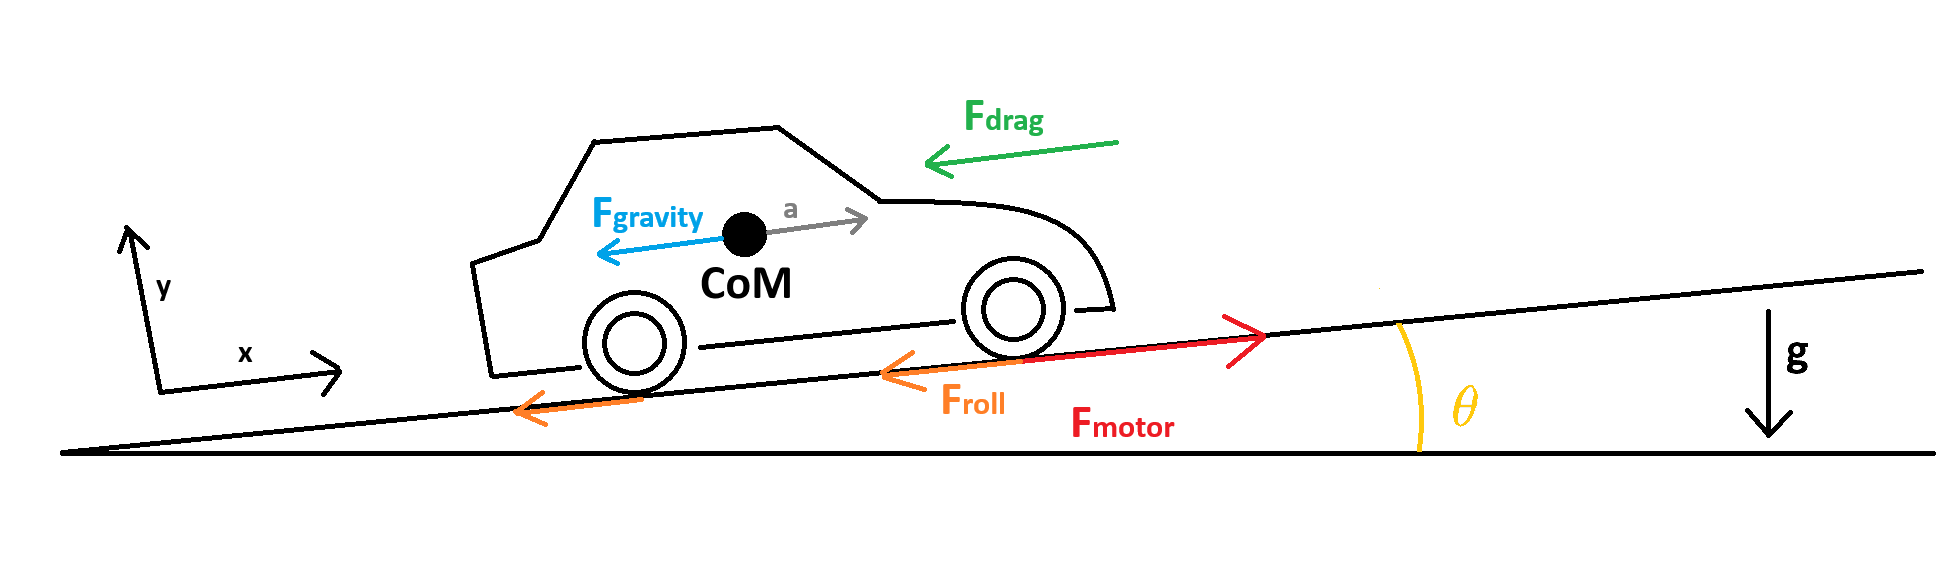
\includegraphics[width=1\linewidth]{Figures/ch1_ForceAxis.png}
    \caption{Longitudinal car dynamics}
    \label{fig:longcardynamics}
\end{figure}

To model the energy requirements of a vehicle in motion, we begin with the classical longitudinal force balance:

\[
m \cdot a = F_{\text{motor}} - F_{\text{drag}} - F_{\text{roll}} + F_{\text{gravity}}
\]

This equation expresses Newton’s second law applied to a vehicle moving along a slope, where \( m \) is the vehicle mass and \( a \) its acceleration. The right-hand side aggregates all relevant external forces acting on the vehicle in the direction of travel.

Substituting each component force into the equation, we obtain the fully expanded expression:

\[
m \cdot a = F_{\text{motor}} - \frac{1}{2} \rho\, C_d\, A\, v^2 - C_{rr}\, m\, g + m\, g\, \sin\theta
\]

This relation captures the competing effects of propulsion, aerodynamic drag, rolling resistance, and gravitation trough road slope. Each parameter affect directly energy consumption.

\vspace{0.5em}
\noindent
\textbf{Definition of Parameters:}
\begin{align*}
m &:\ \text{vehicle mass [kg]} \\
a &:\ \text{longitudinal acceleration [m/s}^2\text{]} \\
F_{\text{motor}} &:\ \text{force produced by the motor or absorbed by braking [N]} \\
\rho &:\ \text{air density [kg/m}^3\text{]} \\
C_d &:\ \text{aerodynamic drag coefficient [–]} \\
A &:\ \text{frontal area of the vehicle [m}^2\text{]} \\
v &:\ \text{vehicle speed [m/s]} \\
C_{rr} &:\ \text{rolling resistance coefficient [–]} \\
g &:\ \text{gravitational acceleration [m/s}^2\text{]} \\
\theta &:\ \text{road slope angle [rad]} \\
\end{align*}

Note that the gravitational term becomes negative when descending (\(\theta < 0\)) and positive when climbing. While the average gravitational contribution over a round trip cancels out, energy losses due to braking and powertrain inefficiencies remain.

Based of the previous equation, we can define the efficiency as 
\begin{equation}
\eta(v) = \left( \frac{1}{2} \rho\, C_d\, A\, v^2 + C_{rr}\, m\, g \right) \quad \text{[N]}
\label{eq:energy_consumption}
\end{equation}

Equation~\eqref{eq:energy_consumption} reveals key design levers: mass \(m\), frontal area \(A\), drag coefficient \(C_d\), and rolling resistance \(C_{rr}\). This simplified model excludes transients like acceleration, braking, wind gusts, and idling, as well as the embodied energy of the vehicle and powertrain losses, which are addressed next.

\subsection{Driving Patterns: Beyond the Idealized Model}

Real-world driving involves multiple phases, each with distinct energy characteristics: cruising, accelerating, braking, and idling. Empirical studies (e.g., \cite{ma_real-world_2019}) provide typical phase distributions over urban trips:

\begin{figure}[h!]
    \centering
    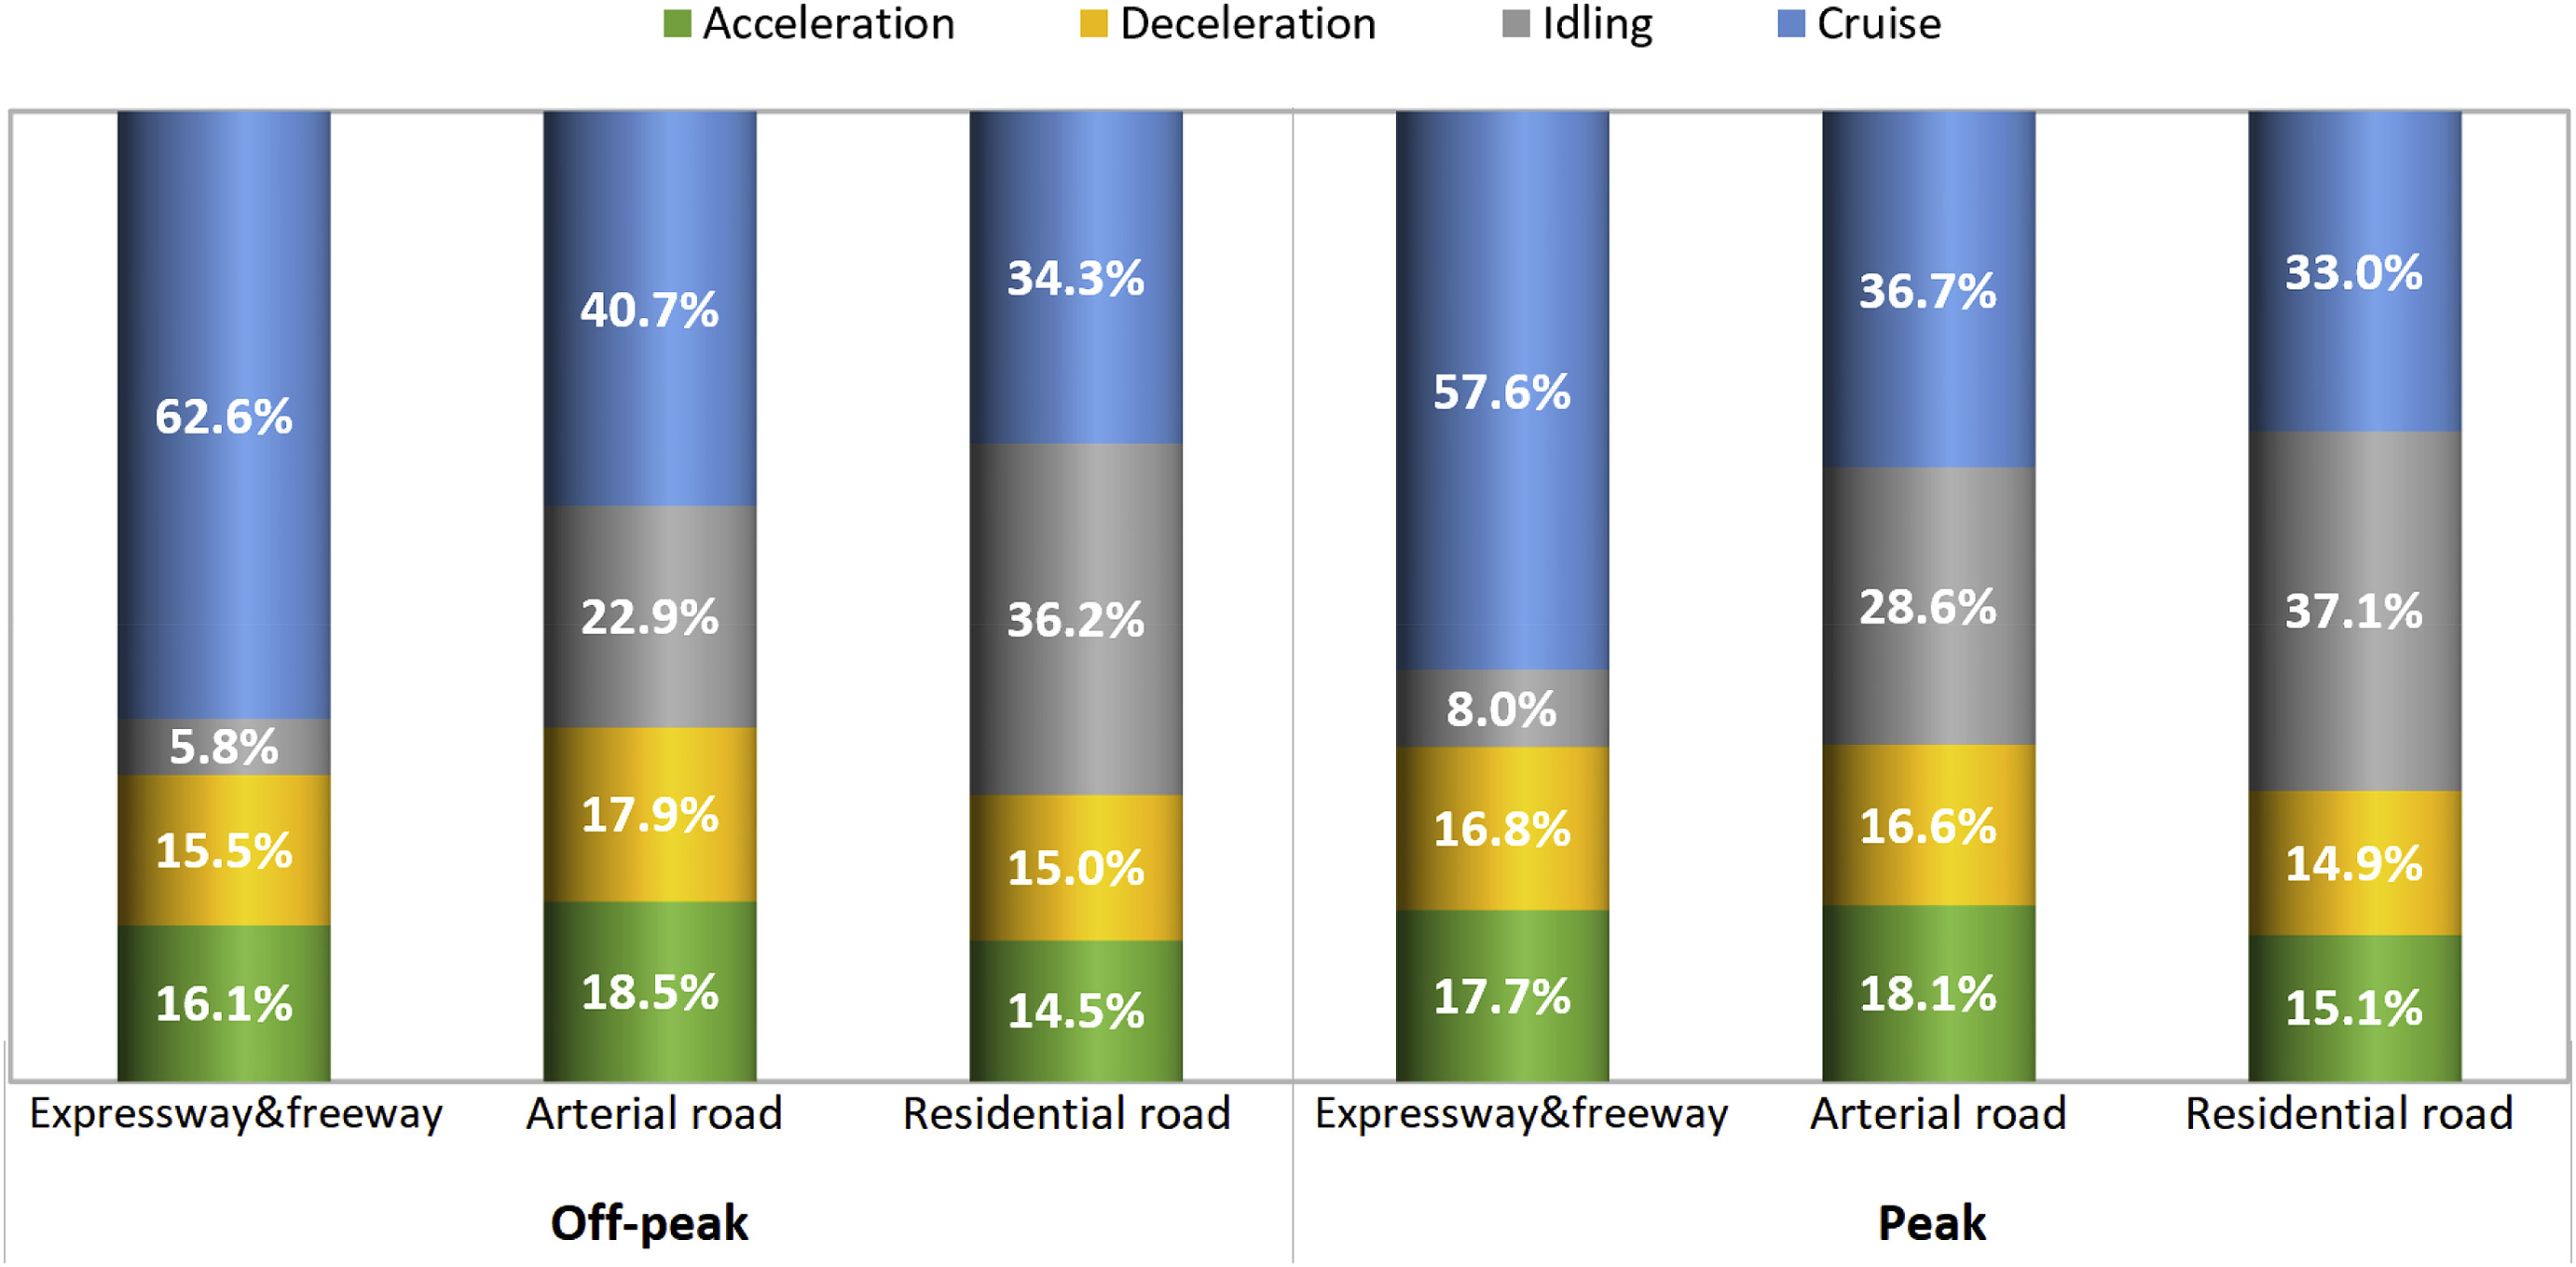
\includegraphics[width=0.7\linewidth]{Figures/ch2_shareOfDrivingModeChina.jpg}
    \caption{Proportion of driving phases during urban operation (Source: \cite{ma_real-world_2019})}
    \label{fig:ch2proportiondrivingmode}
\end{figure}

\newpage 

Most trips in Europe are short, with 80\% under 10 km and 22 minutes \cite{donati_individual_2015}, reinforcing the relevance of frequent transient phases and vehicle warm-up times, especially for Internal Combustion Engine Car (ICE). Trips powered by human effort becomes a plausible benchmark for energy use over such durations.

\begin{figure}[h!]
    \centering
    \subfloat{
        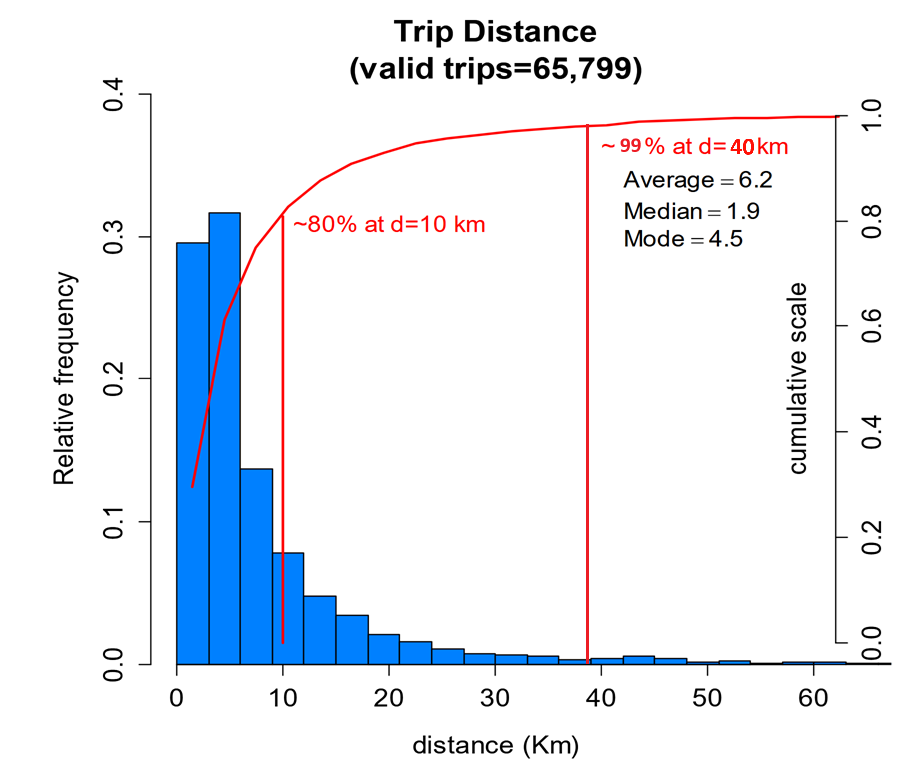
\includegraphics[width=0.45\linewidth]{Figures/ch2_TripsLenghtFrequency.png}
        \label{fig:trips-length}
    }
    \hfill
    \subfloat{
        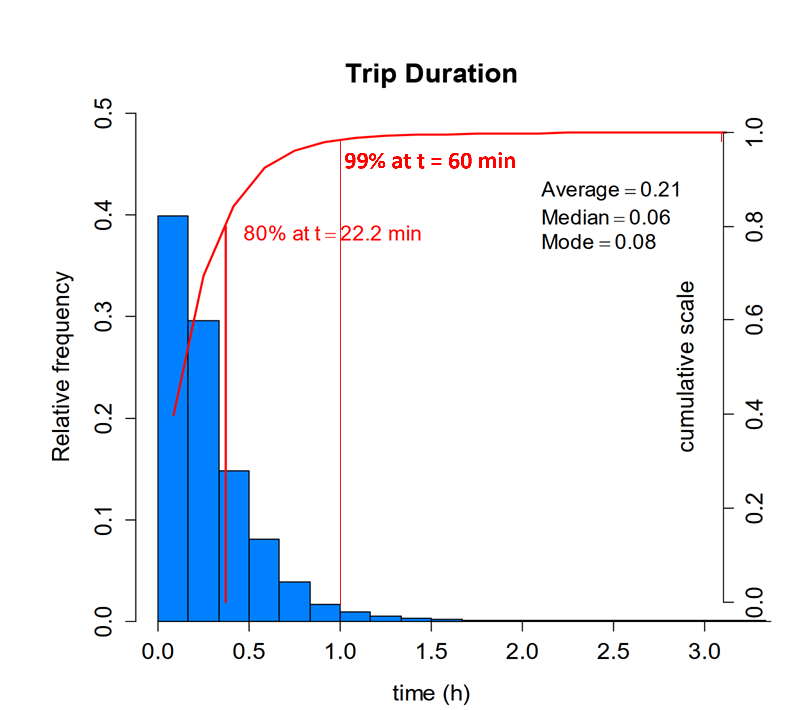
\includegraphics[width=0.45\linewidth]{Figures/ch2_TripsDurationFrequency.png}
        \label{fig:trips-duration}
    }
    \caption{Trip length and duration distributions in Europe (Source: \cite{donati_individual_2015})}
    \label{fig:trips-comparison}
\end{figure}

We define distinct phase efficiencies:

\begin{itemize}
    \item \textbf{Idling Efficiency:} Energy consumed per unit time when stationary. Typically:
    \begin{itemize}
        \item ICE: ~12 kW
        \item EV: $\leq$ 0.5 kW
    \end{itemize}

    \item \textbf{Braking/Deceleration Efficiency:} Energy recovered during braking.
    \begin{itemize}
        \item ICE: 0\%
        \item EV (regen): 50–70\% \cite{noauthor_regenerative_nodate}
    \end{itemize}

    \item \textbf{Acceleration Efficiency:} Energy transferred from tank/battery to kinetic motion.
    \begin{itemize}
        \item ICE: ~13\%
        \item EV: up to 80\% \cite{lohse-busch_ambient_2013}
    \end{itemize}
\end{itemize}

These phase-specific efficiencies reinforce the importance of designing for all driving modes, especially in urban environments characterized by frequent starts and stops.

\subsection{Embodied Energy and Material Impact: Why Mass Matters}

Although this work does not perform a full lifecycle analysis, it is important to acknowledge that manufacturing represents a non-negligible share of a vehicle’s total emissions especially for EVs with energy-intensive battery production. As grid carbon intensity decreases, manufacturing emissions become the limiting factor.

A low-mass, long-lived vehicle, built from materials with low embodied energy, offers a clear advantage in this regard.

\newpage 

\subsection{Parameters Affecting Efficiency}

From Eq.~\eqref{eq:energy_consumption}, we identify key parameters influencing operational energy efficiency:

\begin{itemize}
    \item Reduce \textbf{mass} \(m\) to minimize both rolling resistance and gravitational load.
    \item Minimize \textbf{frontal area} \(A\) and optimize \textbf{drag coefficient} \(C_d\).
    \item Lower the \textbf{rolling resistance coefficient} \(C_{rr}\) via tire selection and surface optimization.
    \item Maximize \textbf{powertrain efficiency} to reduce losses during acceleration and regenerative braking.
    \item Improve \textbf{idling efficiency}, especially critical for short, stop-start urban trips.
\end{itemize}

\subsection{Aerodynamic Optimization Through Form Factor}

Compact, narrow vehicle designs naturally limit frontal area \(A\). Reclined seating and tandem configurations can further reduce the product \(C_d A\), though this introduces challenges related to comfort and accessibility.

\begin{figure}[h!]
    \centering
    \subfloat{
        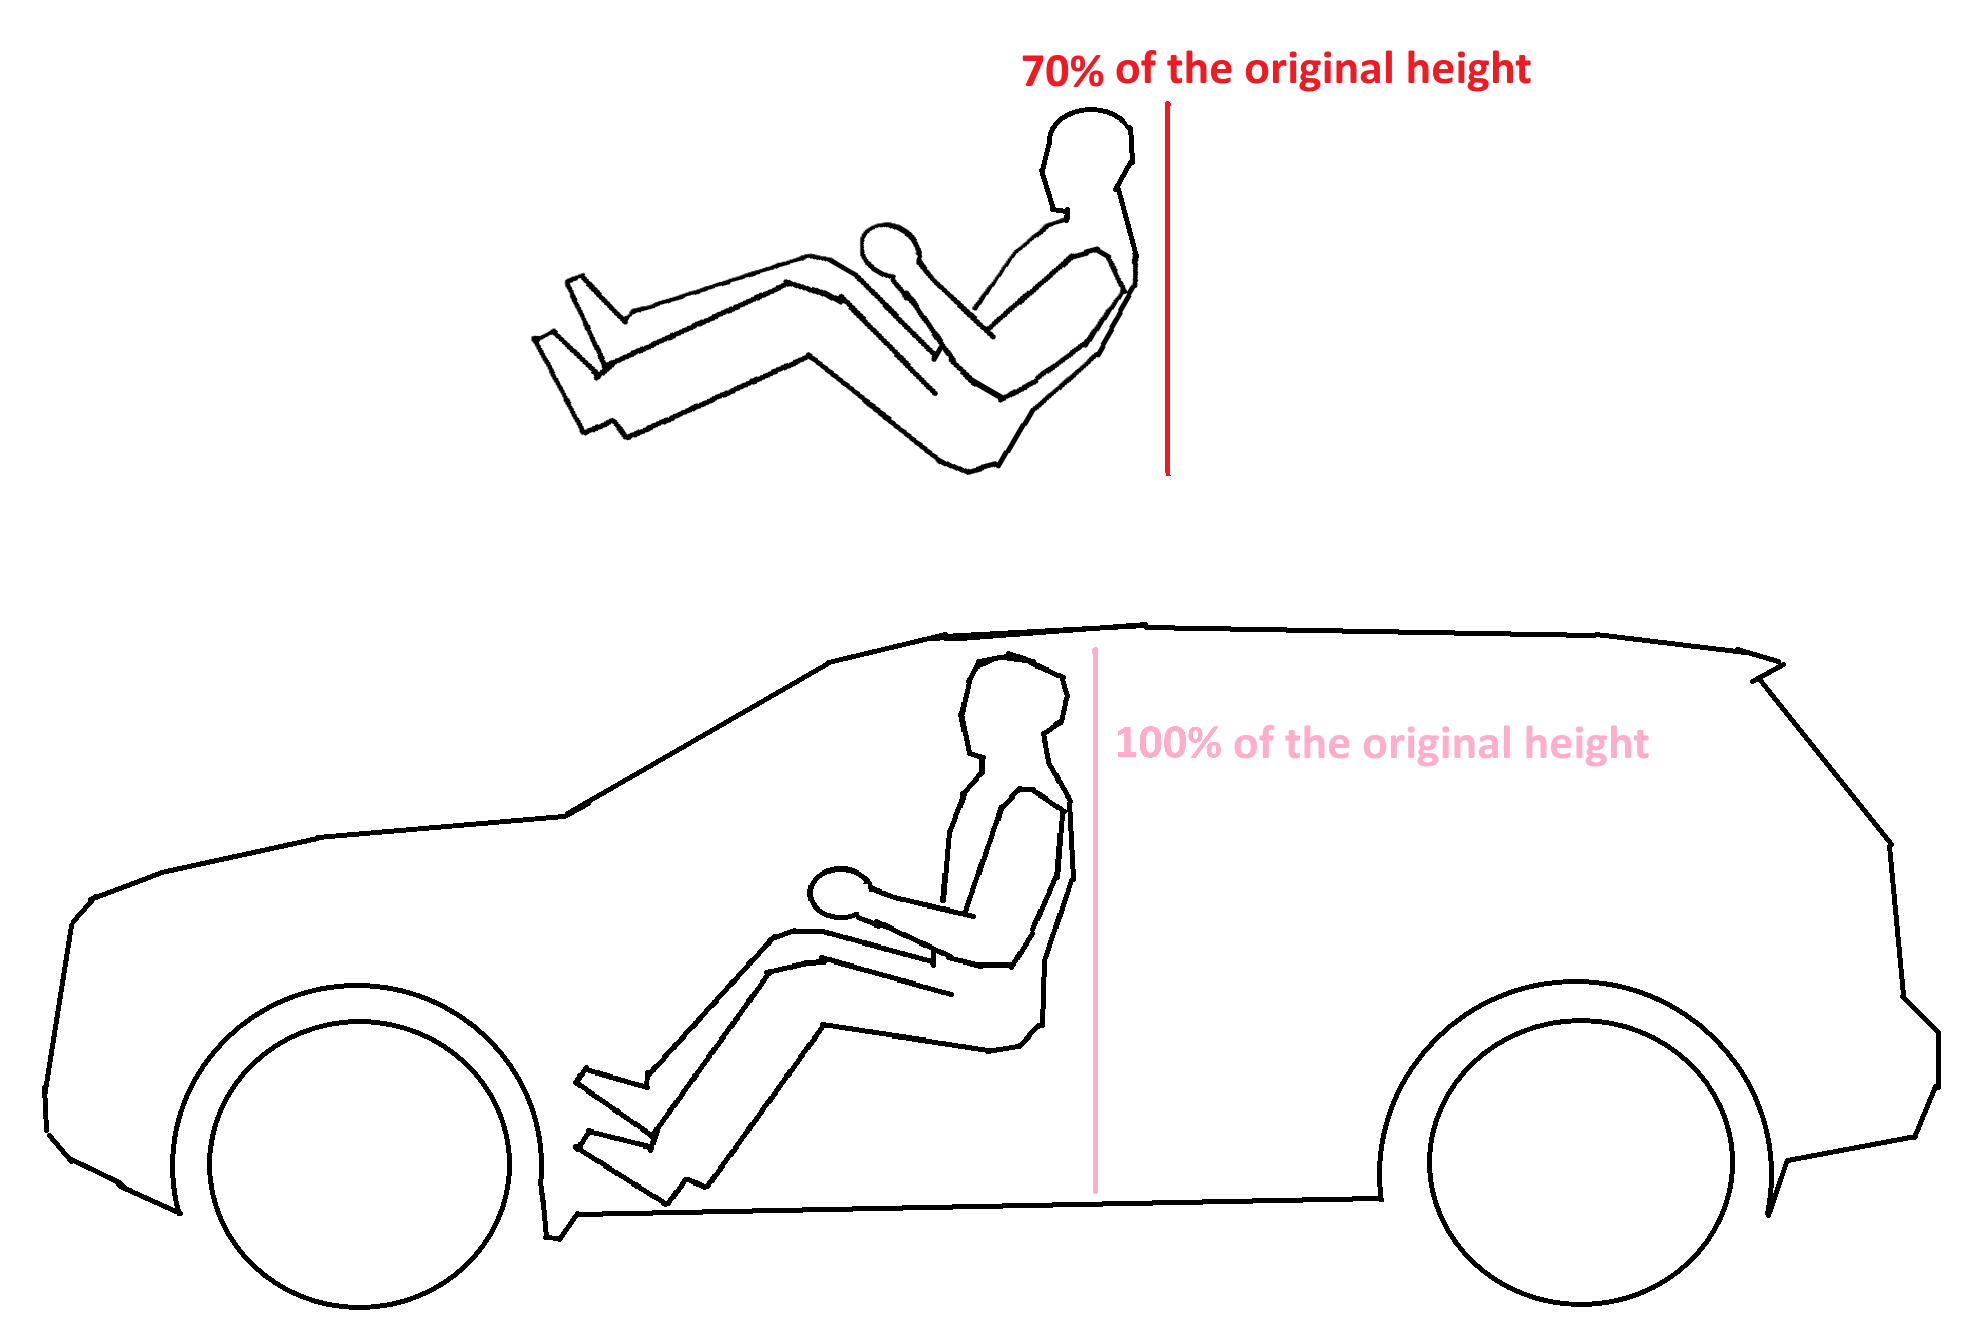
\includegraphics[width=0.47\linewidth]{Figures/ch3_seatingOptimisation.png}
    }
    \hfill
    \subfloat{
        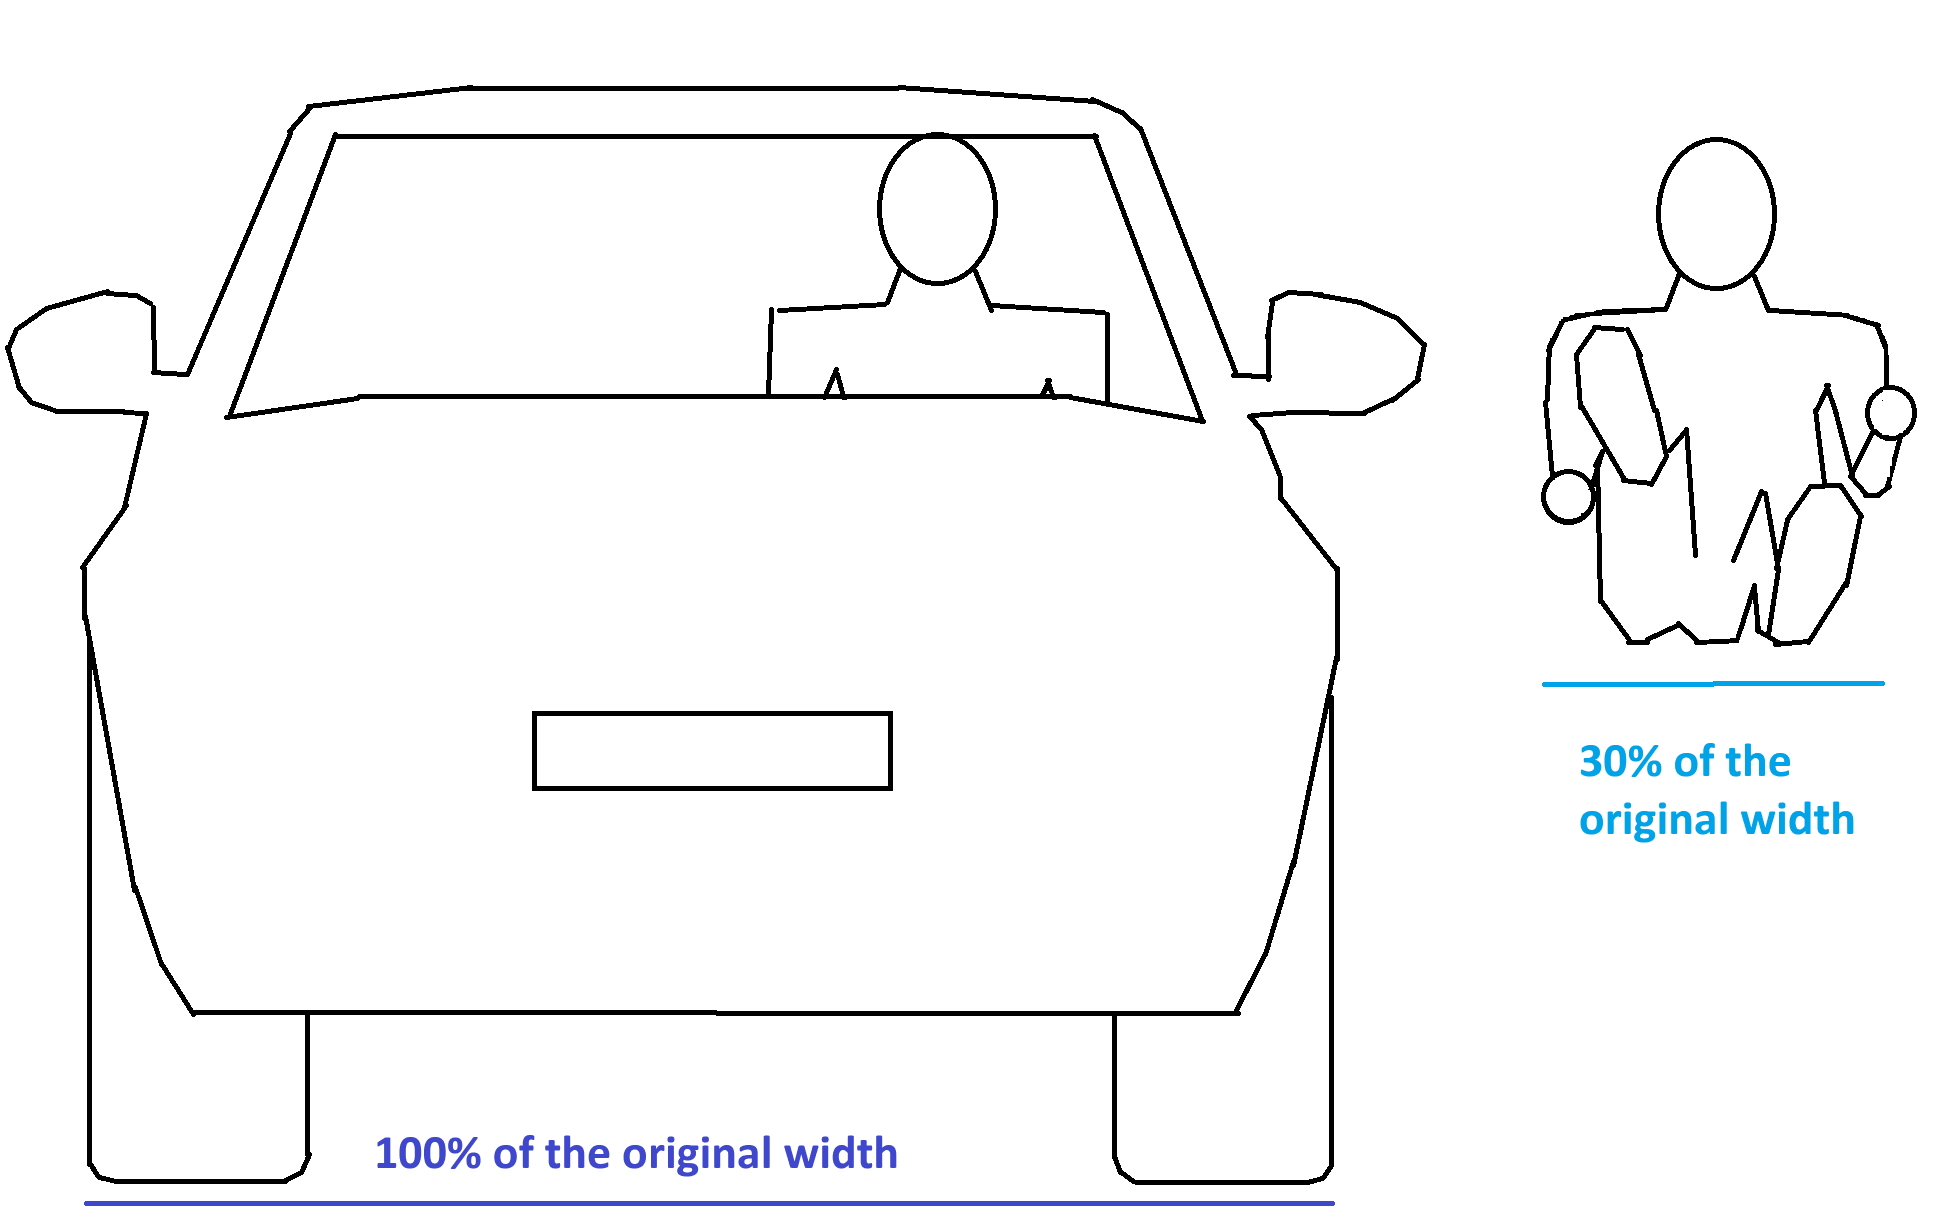
\includegraphics[width=0.47\linewidth]{Figures/ch3_seatingOptimisationFront.png}
    }
    \caption{Effect of seat recline and tandem seating on frontal area}
    \label{fig:FrontaAreaGraphicsComparison}
\end{figure}

Digital augmentation (cameras, screens) could replace traditional visibility elements to further reduce \(A\), but may induce motion sickness due to visual-vestibular mismatches. A partially reclined posture with direct external visibility is a pragmatic compromise.

\begin{figure}[h!]
    \centering
    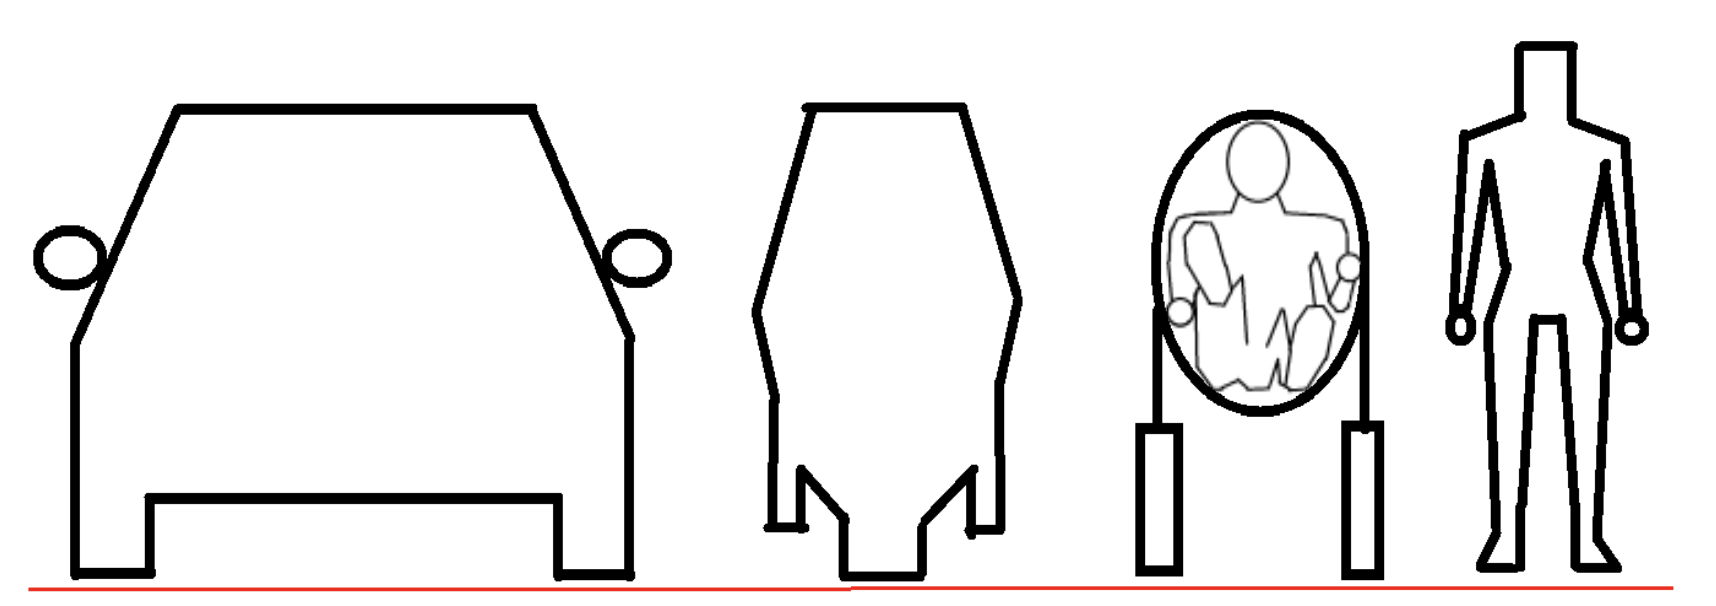
\includegraphics[width=0.8\linewidth]{Figures/ch4_frontComparisonVehicle.png}
    \caption{Frontal area comparison of car, leaning vehicle, proposed concept, and a standing person}
    \label{fig:frontal_comparison}
\end{figure}

Our proposed design incorporates a height-adjustable wheel system, enabling both dynamic tilt control and variable ingress/egress configurations combining aerodynamic form with accessibility.


\section{Design Considerations}

\subsection{Reducing Frontal Area and improving the coefficient of drag}
look at how many passengers per vehicle on average trips, the seating layout and its implication on the aerodynamics.

look at how to reduce frontal area by seating position

\subsection{Reducing mass and embodied energy}
why are car heavy ? what is energy intensive in a car ?

\subsection{Addressing Visibility and Safety Concerns in Traffic}

why trike and velomobile are not more mainstream (economics and  driving lower than anybody else, more ?)

\subsection{User comfort requirement}
(thermal, noise, water ingress, seating position)
study about what people need in car. we are we sensitive about when travelling / commuting

\subsection{Narrow Track and Low Vehicle Geometry (literature review)}
Acknowledge existing solution
\section{Innovative Design Concept}

\subsection{Elevating the Vehicle Without Increasing Frontal Area}

Current approach tend to have the vehicle body occupy the whole front area and utilize this space to house the leaning system. Instead, we will focus on an active swing arm design with passive caster wheel. The act of leaning will force the wheel to turn in the wanted direction. This arrangement offer the advantage of occupying less frontal area while allowing to raise and lower the vehicle to both improve visibility in traffic and facilitate entrance and exit.

Make a drawing with the cabin + passenger and wheel. show the design space.

Design 0 : tilting cabin, show the occupied space

design A : 2 front arm along body, passive wheel to turn, one fixed wheel behind

design B : 2 front arm along body, passive wheel to turn, 2 wheel on two arm behind.

design C : 2 front arm sideways crab of body, passive wheel to turn, one fixed wheel behind

design D : 2 front arm sideways crab of body, passive wheel to turn, one fixed wheel behind

design E : 2 front arm sideways crab of body + suspension vertical, passive wheel to turn, one fixed wheel behind

design F : 2 front arm sideways crab of body + suspension vertical, passive wheel to turn, 2 wheel on arm behind

design G : 2 front arm, lateral extension of body + suspension vertical, passive wheel to turn, one fixed wheel behind

design H : 2 front arm lateral extension of body + suspension vertical, passive wheel to turn, 2 wheel on arm behind

design I : 2 front arm lateral extension of body + suspension vertical, two passive wheels to turn behind

design J : 2 front wheel with passive pivot, arm lateral extension of body + suspension vertical and powered motor behind

design H : 1 front wheel with passive pivot. Dual arm lateral extension of body + suspension vertical and powered motor behind

design I : 1 rear wheel with passive pivot. Dual arm lateral extension of body + suspension vertical and powered motor in front


from previous chapter, want to lower frontal area while keeping user eyes high from the ground\\

how can we do so on a kinematic standpoint, and what synergies can we gain from coupling the steering to the leaning ?\\

Use wheel to help control, differential speed\\

3 wheel 1 front -> \\
3 wheel 2 front -> \\
4 wheel         -> \\

Tilting body, \\
plunging wheel, \\
(arm)\\

Free to Roll\\
Free to caster\\
Active control\\

*** steering approach\\
-> skid steer\\
-> ackerman\\
-> swerve wheel + crab steering\\
-> 2 wheel lean to steer (trail + no trail ?)\\
-> other\\
*** geometry and kinematic\\
-> vertical actuator\\
-> arm along vehciule\\
-> arm sideways vehicule\\
-> others ?\\


Wheel, contact patch, function of camber angle on Self-Aligning Torque\\
wheel, gyroscope, \\
wheel, mass and shock absorption \\
Fork Offset, effect on Self-Aligning Torque\\



\subsection{Benefits for Vertical Parking and Accessibility}
talk about the advantage of the selected design, how it could park vertically and what good it would do in city.\\

compare to a normal car, show what would happen if it can park 6 time more. talk about rebound effect risk.

talk about the stability while boarding and exiting, how the vehicle can help to make it a "normal chair" posture then reclining, frontal entry (lateral feel less stable)\\
front entry for more stability.

\subsection{Integration with Public Transport Infrastructure (e.g., Trains)}
possible advantage of loading the vehicle on train for high speed, long distance travel. could beat both car and public transport ? light enough to be lifter by a person  and small enough to occupy roughly the same footprint as a bike.
\section{Dynamic Analysis}

-> test with simple bycycle, show behavior, try to see the counter steer thing ?\\ (counter steering to innitiate leaning moment, less control action)

-> how does it behave on straight road ( with bump and or not flat) ?\\

-> how does it behave during cornering (road with bump and not flat)

-> relationship spring to negate effect of weight and weight change ?\\

\subsection{Prevention of Tipping During Turns}

\subsection{Stability on the Road: Key Parameters and Insights}

\subsection{Comparison of Steering and Leaning Systems}

\subsection{Energy efficiency}
TODO IF TIME : 
we can if we have time use the markov process and integrate of the efficiency over many trips to have an average trip efficiency and have some weight.

also get some number on the acceleration braking amount and quantity (how much and how many) (use markov model (1 seconde per state and compare with gofar data for braking)

\subsection{Travel time}
It's also interesting to look at the speed profile on road to define how fast the vehicle need to go (as required by real world data) and the tradeoff between trip time and speed if we have to cap the max speed (at let's say 60 kmh). (effect should be manageable since little time is spent at autobahn speed.

get a number on the impact of the vehicle performance on trip duration.

\section{Proposed Designs}
Our design aims to retain the high energy efficiency potential demonstrated in Section~2, while integrating the urban constraints discussed in Section~3 and the user requirements outlined in Section~4. The result is a narrow, lightweight, enclosed vehicle assimilated to a cycle.

\textbf{1. Efficiency:}  
By minimizing mass and frontal area, using low rolling resistance wheels, and optimizing aerodynamics (target $C_d \approx 0.15$), the proposed vehicle matches the energy performance of state-of-the-art velomobiles and outperforms an electric car and an ICE car by a factor 10 and 50 respectively on an efficiency level.

\textbf{2. Human experience:}  
Unlike velomobiles or e-bikes, this concept improves rider visibility and perceived safety by raising the riding position without compromising stability, thanks to a leaning mechanism. This system also simplifies ingress and egress (the vehicle tilts forward to assist the user) and allows for vertical parking, improving usability in dense urban settings.

\textbf{3. Urban compatibility:}  
The vehicle occupies far less road and parking space than a car, and remains legally within bicycle limits, allowing access to bike lanes while being able to keep up with traffic pace.

\vspace{0.3em}

Although existing solutions will be examined in more detail further, we can already see that :  \\
\textbf{E-bikes and velomobiles} often come short from a user standpoint as they fail to address minimal comfort and safety requirement.
While \textbf{Cars}, on the other hand, fail on efficiency and urban integration by being oversized in both energy and space usage.

Here are presented the two main parameters of the design space that we will study on a dynamic standpoint : the choice between a three or four-wheel configuration (figure \ref{fig:number_of_wheel}), and two leaning mechanisms (figure \ref{fig:leaning_mechanism}) that use either pivot arm vs. linear-guided suspension to ensure stability while enabling an elevated riding position. 

Figure \ref{fig:vertical_parking_easy_egress} highlight how the proposed layout benefit egress/ingress and vertical storage by allowing to recline the seat and let the user easily redress the vehicle.


\begin{figure}[h!]
    \centering
    \begin{minipage}{0.45\linewidth}
        \centering
        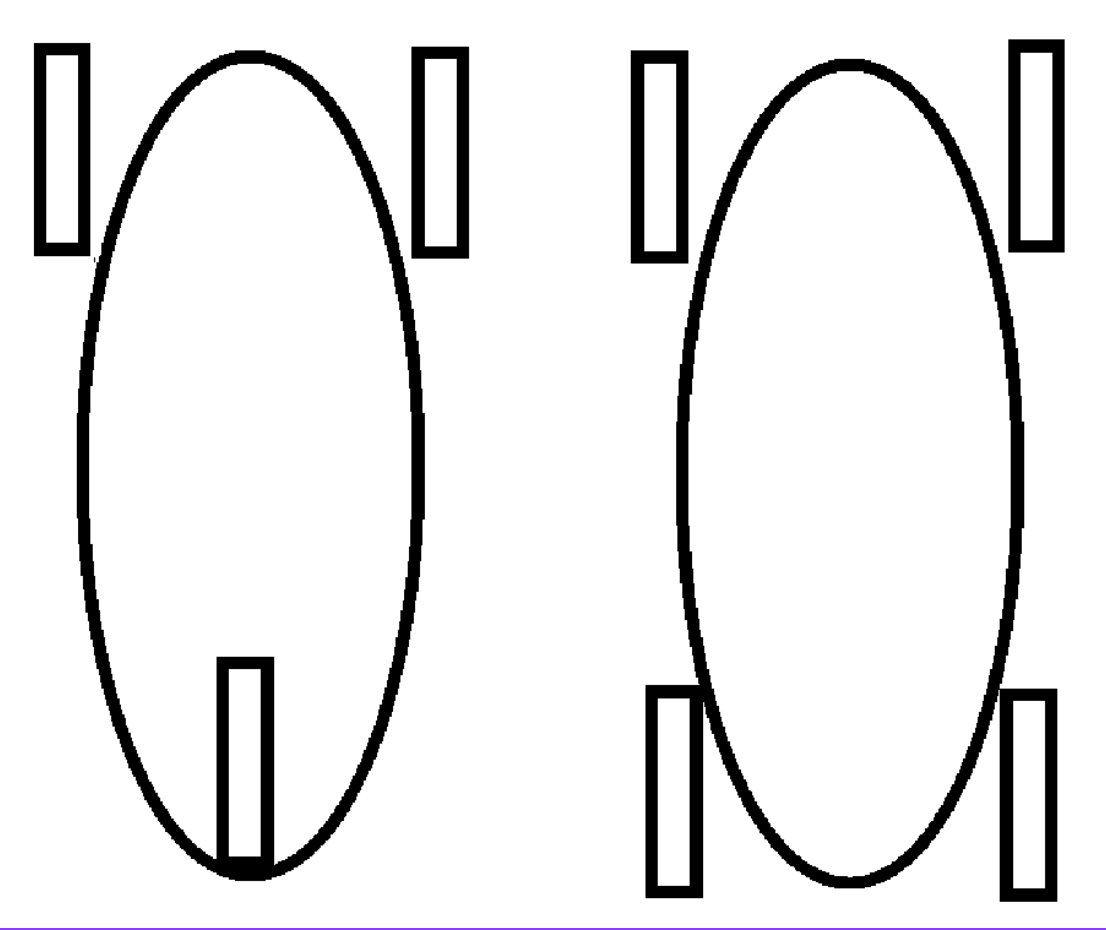
\includegraphics[width=\linewidth]{Figures/ch4_three_vs_four_wheel.png}
        \caption{Three and Four wheeler configuration}
        \label{fig:number_of_wheel}
    \end{minipage}
    \hfill
    \begin{minipage}{0.35\linewidth}
        \centering
        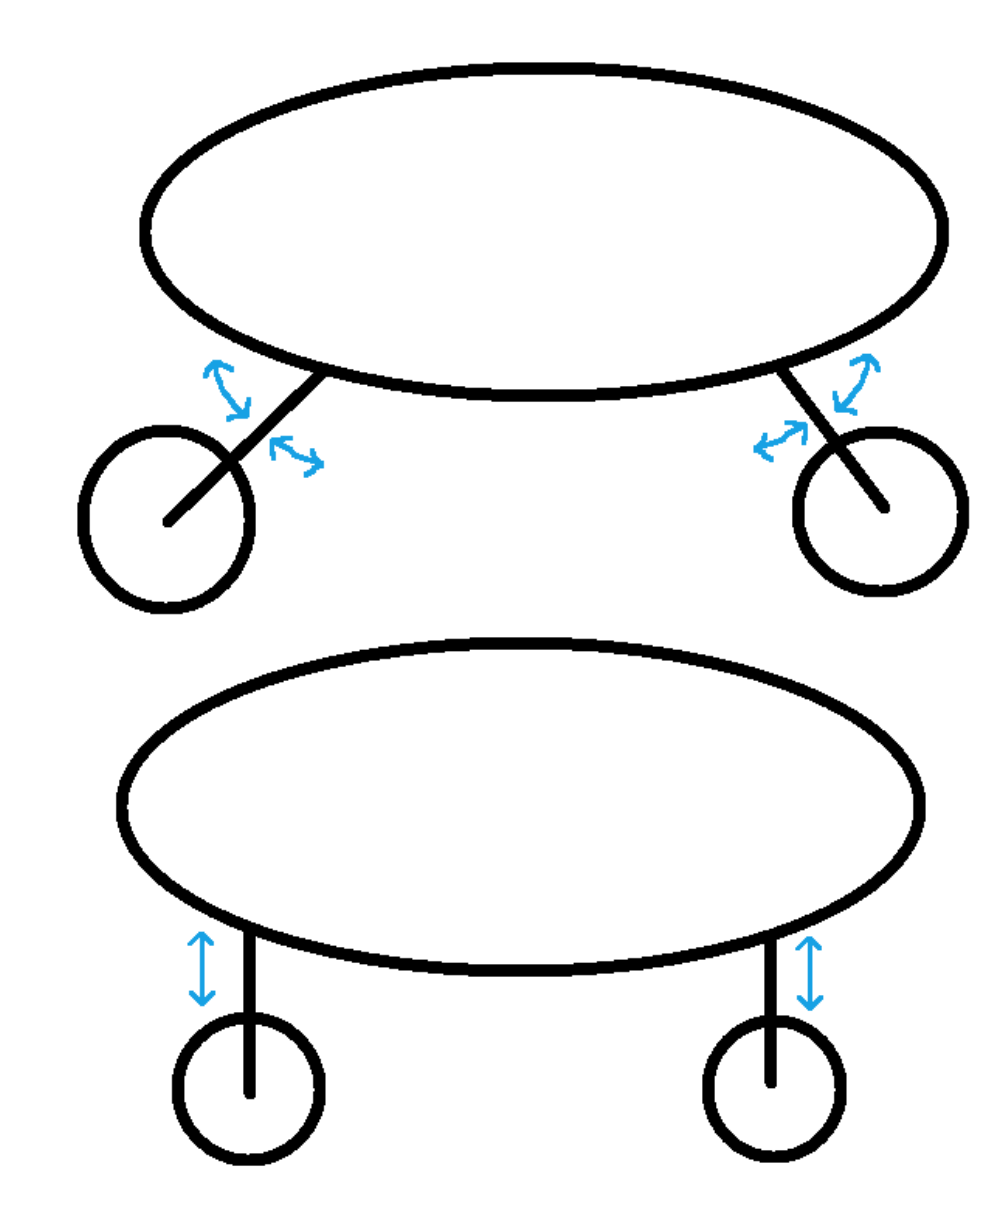
\includegraphics[width=\linewidth]{Figures/ch4_WheelMechanismHeightAdaption.png}
        \caption{Leaning mechanism based either on a pivot or a linear-guided suspension}
        \label{fig:leaning_mechanism}
    \end{minipage}
\end{figure}

\newpage 

\begin{figure}[h!]
    \centering
    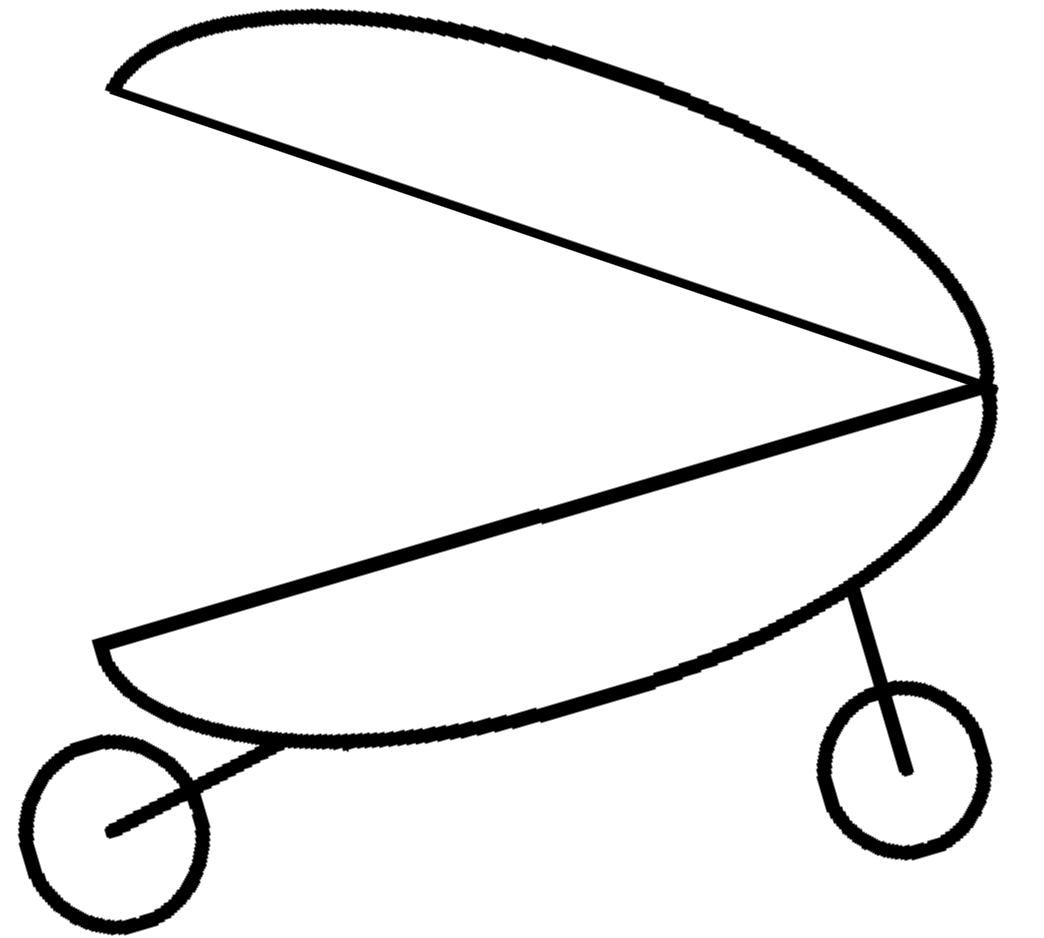
\includegraphics[width=0.5\linewidth]{Figures/ch4_EgressReclining.png}
    \caption{Simplified Egress and vertical parking}
    \label{fig:vertical_parking_easy_egress}
\end{figure}

\vfill


\subsection{Comparative Evaluation}
The proposed design consistently scores higher across efficiency, urban integration, and human experience compared to both cars and cycle-based alternatives. By combining a compact footprint with enhanced protection and usability, it bridges the gap between comfort and sustainability. However, this performance comes at the cost of increased mechanical and control complexity, inherent to narrow-track vehicles. To address these challenges, we will evaluate multiple mechanical configurations including three-wheel and four-wheel variants, as well as different leaning actuation strategies based on linear actuators or pivot mechanisms. These configurations will be analyzed both from a static standpoint to assess tipping stability and from a dynamic perspective. The following chapters will dive into these aspects, starting with the analysis of static behavior before transitioning to the more demanding problem of dynamic stabilization and control.

\newpage 

\begin{table}[h!]
\caption{Performance Comparison}
\centering
\renewcommand{\arraystretch}{1.25}
\setlength{\tabcolsep}{5pt}
\begin{tabularx}{\textwidth}{lXXXXX}
\toprule
\textbf{Parameter} & \textbf{E-Bike} & \textbf{Velomobile} & \textbf{ ICE Car} & \textbf{Electric Car} & \textbf{Proposed Design} \\
\midrule
\multicolumn{6}{l}{\textbf{Section 1: Efficiency}} \\
Drive train efficiency        & \cellcolor{LightGreen}$\geq70\%$     & \cellcolor{LightGreen}$\geq70\%$     & \cellcolor{LightRed}$\leq30\%$       & \cellcolor{LightGreen}$\geq80\%$     & \cellcolor{LightGreen}$\geq80\%$ \\
$C_d$ (drag coefficient)      & \cellcolor{LightRed}1                & \cellcolor{LightGreen}0.15           & \cellcolor{LightRed}0.3              & \cellcolor{LightOrange}0.2           & \cellcolor{LightGreen}0.15 \\
Frontal area (m²)            & \cellcolor{LightGreen}0.5            & \cellcolor{LightGreen}0.35           & \cellcolor{LightRed}2.3              & \cellcolor{LightRed}2.3              & \cellcolor{LightGreen}$\leq$0.7 \\
Mass $m$ (kg)                & \cellcolor{LightGreen}85             & \cellcolor{LightGreen}110            & \cellcolor{LightRed}1100             & \cellcolor{LightRed}1300             & \cellcolor{LightGreen}$<$250 \\
$C_{rr}$ (rolling resistance) & \cellcolor{LightGreen}0.004          & \cellcolor{LightGreen}0.004          & \cellcolor{LightOrange}0.01          & \cellcolor{LightOrange}0.01          & \cellcolor{LightGreen}0.004 \\
\midrule
\multicolumn{6}{l}{\textbf{Section 2: Urban Elements}} \\
Width (cm)                  & \cellcolor{LightGreen}50             & \cellcolor{LightGreen}70             & \cellcolor{LightRed}180              & \cellcolor{LightRed}180              & \cellcolor{LightGreen}$<$70 \\
Parking space (m²)          & \cellcolor{LightGreen}1              & \cellcolor{LightGreen}1.5            & \cellcolor{LightRed}12               & \cellcolor{LightRed}12               & \cellcolor{LightGreen}$\approx$0.7 \\
Speed (km/h)                & \cellcolor{LightOrange}45            & \cellcolor{LightOrange}45            & \cellcolor{LightGreen}120            & \cellcolor{LightGreen}120            & \cellcolor{LightGreen}60-80 \\
Power-to-weight (continuous) & \cellcolor{LightOrange}13 W/kg       & \cellcolor{LightOrange}10 W/kg       & \cellcolor{LightGreen}50 W/kg        & \cellcolor{LightGreen}60 W/kg        & \cellcolor{LightOrange}$1–25 W/kg^*$ \\
Power-to-weight (peak)       & \cellcolor{LightOrange}16 W/kg       & \cellcolor{LightOrange}13 W/kg       & \cellcolor{LightGreen}50 W/kg        & \cellcolor{LightGreen}120 W/kg       & \cellcolor{LightGreen}60 W/kg \\
\midrule
\multicolumn{6}{l}{\textbf{Section 3: Human Elements}} \\
Feeling visible / high road   & \cellcolor{LightGreen}Good           & \cellcolor{LightRed}Bad              & \cellcolor{LightGreen}Good           & \cellcolor{LightGreen}Good           & \cellcolor{LightGreen}Good \\
Feeling protected             & \cellcolor{LightRed}Poor             & \cellcolor{LightOrange}Fair          & \cellcolor{LightGreen}Good           & \cellcolor{LightGreen}Good           & \cellcolor{LightGreen}Good \\
Physical effort               & \cellcolor{LightOrange}Medium        & \cellcolor{LightOrange}Medium        & \cellcolor{LightGreen}None           & \cellcolor{LightGreen}None           & \cellcolor{LightGreen}minimal \& Constant \\
Cargo \& passenger capacity   & \cellcolor{LightRed}Low              & \cellcolor{LightOrange}Fair          & \cellcolor{LightGreen}Good           & \cellcolor{LightGreen}Good           & \cellcolor{LightGreen}2 adult or 4-5 bag \\
Weather / thermal protection  & \cellcolor{LightRed}Minimal          & \cellcolor{LightGreen}Good           & \cellcolor{LightGreen}Good           & \cellcolor{LightGreen}Good           & \cellcolor{LightGreen}Good \\
Privacy / comfort             & \cellcolor{LightRed}Poor             & \cellcolor{LightOrange}Fair          & \cellcolor{LightGreen}Good           & \cellcolor{LightGreen}Good           & \cellcolor{LightGreen}Good \\
Ease of entry / exit          & \cellcolor{LightOrange}Fair          & \cellcolor{LightRed}Difficult        & \cellcolor{LightGreen}Good           & \cellcolor{LightGreen}Good           & \cellcolor{LightGreen}Front-tilt, upright \\
\bottomrule
\end{tabularx}
\end{table}

\paragraph*{Note on Power-to-Weight Ratio ($^*$):}
The continuous power-to-weight ratio marked with an asterisk refers to the average sustained power a person can provide typically around \textbf{1\,W/kg}. This estimate is sufficient for flat terrain and steady-state cruising, where only aerodynamic and rolling resistance need to be overcome.

While slope climbing and acceleration phases require much higher instantaneous power, up to \textbf{25\,W/kg}. The energy spent climbing is largely recovered when descending. As a result, over the course of a typical ride, elevation changes and accelerations tend to cancel out in terms of net energy expenditure assuming the losses are compensated. 

Therefore, even though higher peak power is occasionally needed, a continuous input of \textbf{1\,W/kg} is generally enough to sustain average cruising performance effectively allowing the user to achieve what would otherwise require a \textbf{25\,W/kg} system, provided that energy buffering (e.g., a battery or gravity) absorbs the transient demands.

\section{Prototype Development}

if we hypothetically wanted to build one, what would it take ?\\

\subsection{Legal requirements}

\subsection{Material Selection and Cost Analysis}

\subsection{Preliminary Design Specifications}

\subsection{Feasibility of Building the Prototype}


\section{Dynamic Behavior and Control}

Tilting Narrow Track Vehicles (NTVs) with a high center of mass (CoM) are inherently unstable, necessitating active stabilization to remain upright and controllable. Due to time constraints, a full dynamic controller is beyond the scope of this work. Instead, we demonstrate the viability of steady-state stabilization using a tuned PID controller to maintain balance during straight-line travel and constant-radius turns. The primary goal is to compare the dynamic response of multiple design variants, specifically 3-wheel versus 4-wheel layouts, and rotational versus linear tilt arm mechanisms, under two representative conditions. This results in a total of 8 simulated scenarios. Each simulation is treated as a steady-state configuration, with basic PID control used to stabilize the lean angle. While this does not capture transient or disturbance responses, it is sufficient to evaluate geometry-dependent trends and identify promising configurations for further development.


\subsection{Methodology}

The simulation framework was built using PyBullet, a real-time physics engine. Each vehicle configuration was modeled using a URDF file that specifies link geometry, mass distribution, and joint constraints. Four base configurations were created by combining two platform layouts (three-wheel and four-wheel) with two leaning mechanisms (pivot-based and linear-guided). Each of these was simulated under two scenarios: straight-line motion and constant-radius turning, yielding eight unique scenarios. The straight line scenario occurred on a bumpy surface, while the Curved scenario operated on a flat surface.

For each configuration, the lean angle was controlled via a custom PID controller implemented in the simulation loop. The system was initialized at rest and brought to a constant velocity. For turning scenarios, a fixed-radius turn was imposed by constraining the trajectory. The controller was responsible for adjusting the lean angle to balance centrifugal forces during turning or gravitational instability during straight-line motion.

All simulations recorded joint states (position, velocity, acceleration) and key global metrics such as vehicle lean angle, lateral deviation, and applied control torque. Screenshots of each configuration were captured to document visual differences and posture under dynamic conditions.

\subsection{Implementation}

Each vehicle model is defined using a modular URDF structure, with separate subtrees for chassis, suspension, and lean mechanism. The joint-level PID controller operates within the PyBullet simulation loop at a frequency of 240 Hz. The control law follows:

\[
\tau = K_p(\theta_{\text{desired}} - \theta) + K_d(\dot{\theta}_{\text{desired}} - \dot{\theta}) + K_i \int (\theta_{\text{desired}} - \theta) \, dt
\]

where $\tau$ is the control torque, $\theta$ is the lean joint state, and $\dot{\theta}$ is its velocity. Gains $K_p$, $K_i$, and $K_d$ were manually tuned for each configuration to achieve stable convergence and minimize oscillation.

Data was logged for plotting and post-processing. Camera control was implemented to enable 3D inspection of vehicle motion and stability during runtime, facilitating visual validation of lean behavior and dynamic posture. The figure \ref{fig:actuator-configs} show how the different configuration were implemented in pybullet. The Base mass was set to 100 [kg] while the wheel and segment mass were set to 1 [kg] to emphasize the high CoM.

\newpage

\begin{figure}[h!]
    \centering
    \begin{subfigure}[b]{0.45\linewidth}
        \centering
        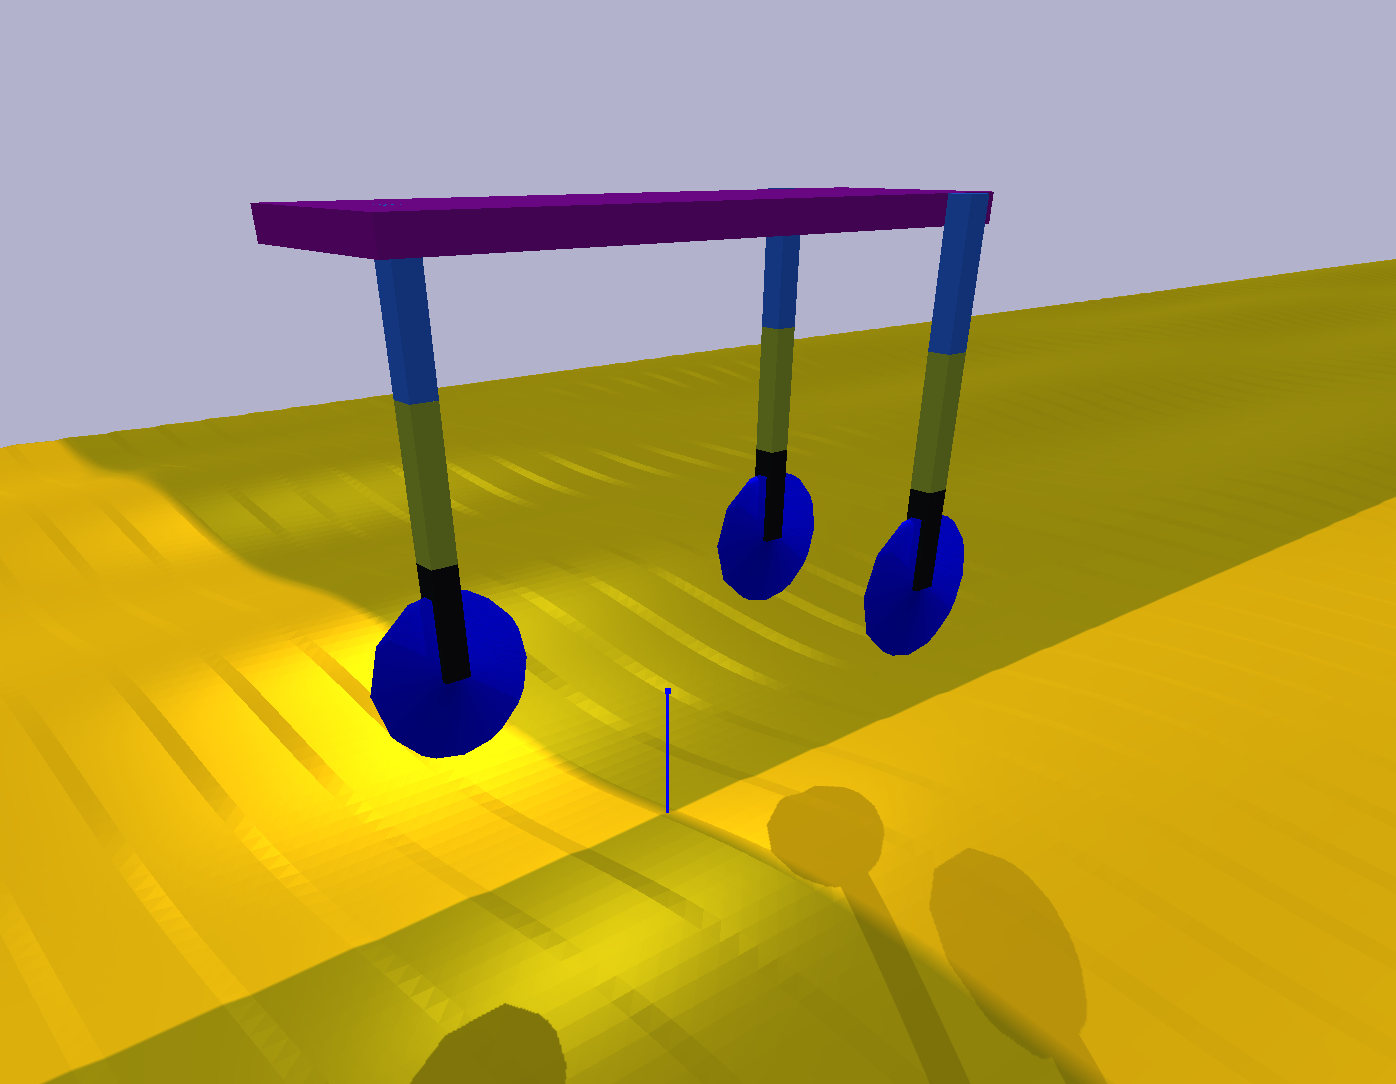
\includegraphics[width=\linewidth]{Figures/ch8_LinearThreeWheel.png}
        \caption{Three Wheeler With Linear Actuator}
    \end{subfigure}
    \hfill
    \begin{subfigure}[b]{0.45\linewidth}
        \centering
        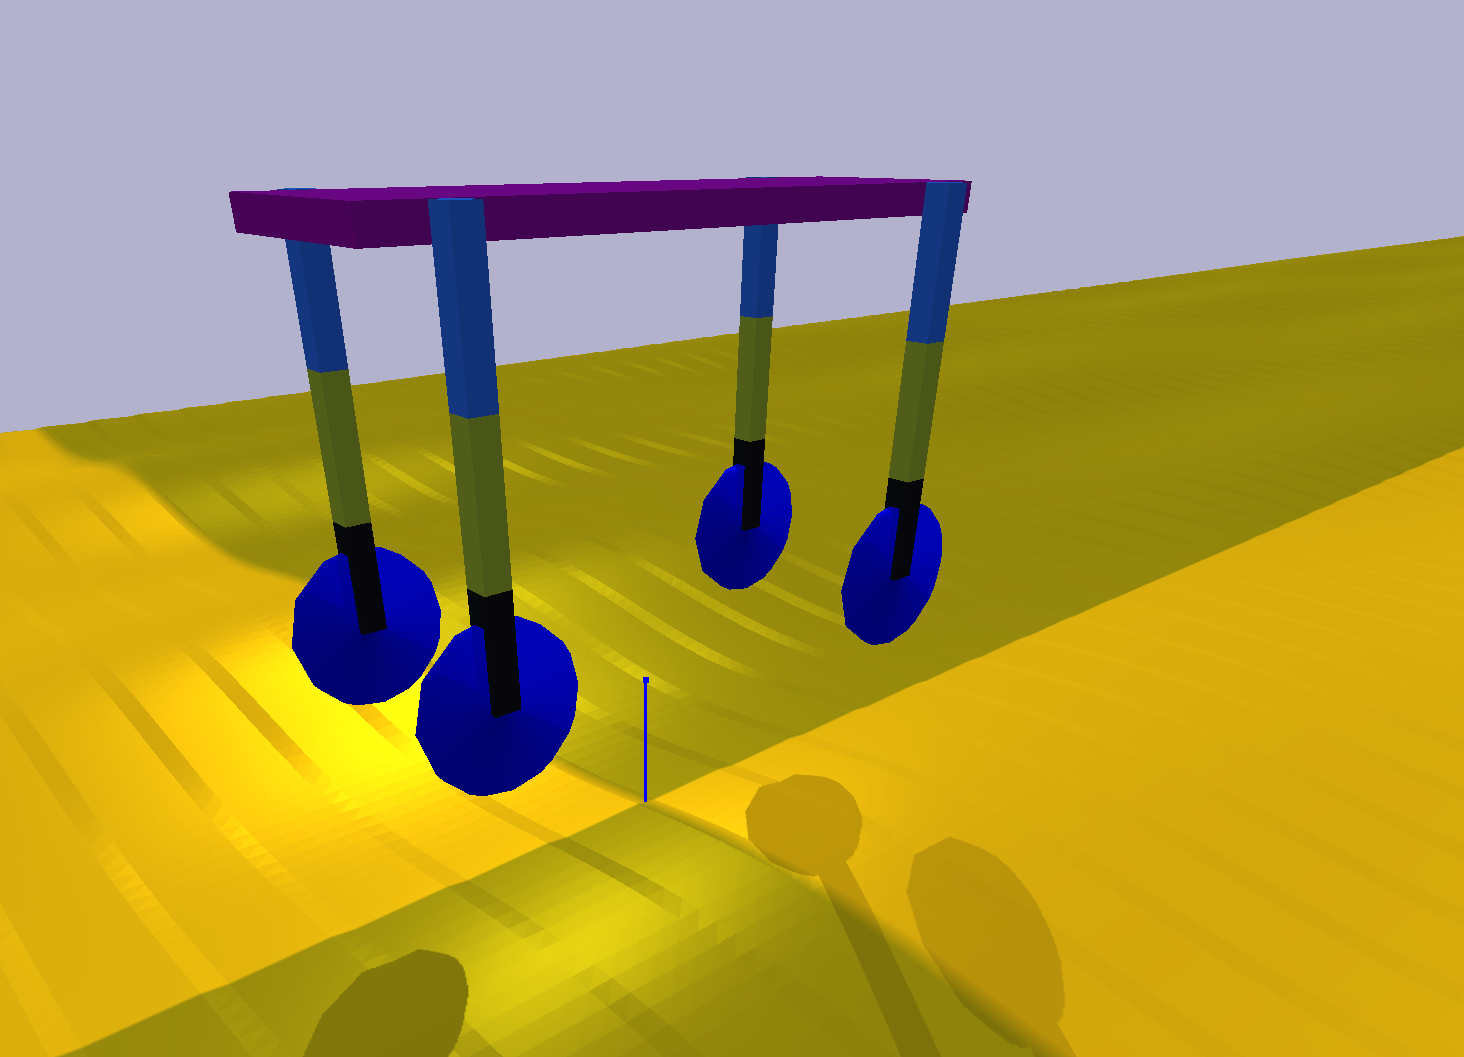
\includegraphics[width=\linewidth]{Figures/ch8_LinearFourWheel.png}
        \caption{Four Wheeler With Linear Actuator}
    \end{subfigure}
    
    \vspace{0.5cm}
    
    \begin{subfigure}[b]{0.45\linewidth}
        \centering
        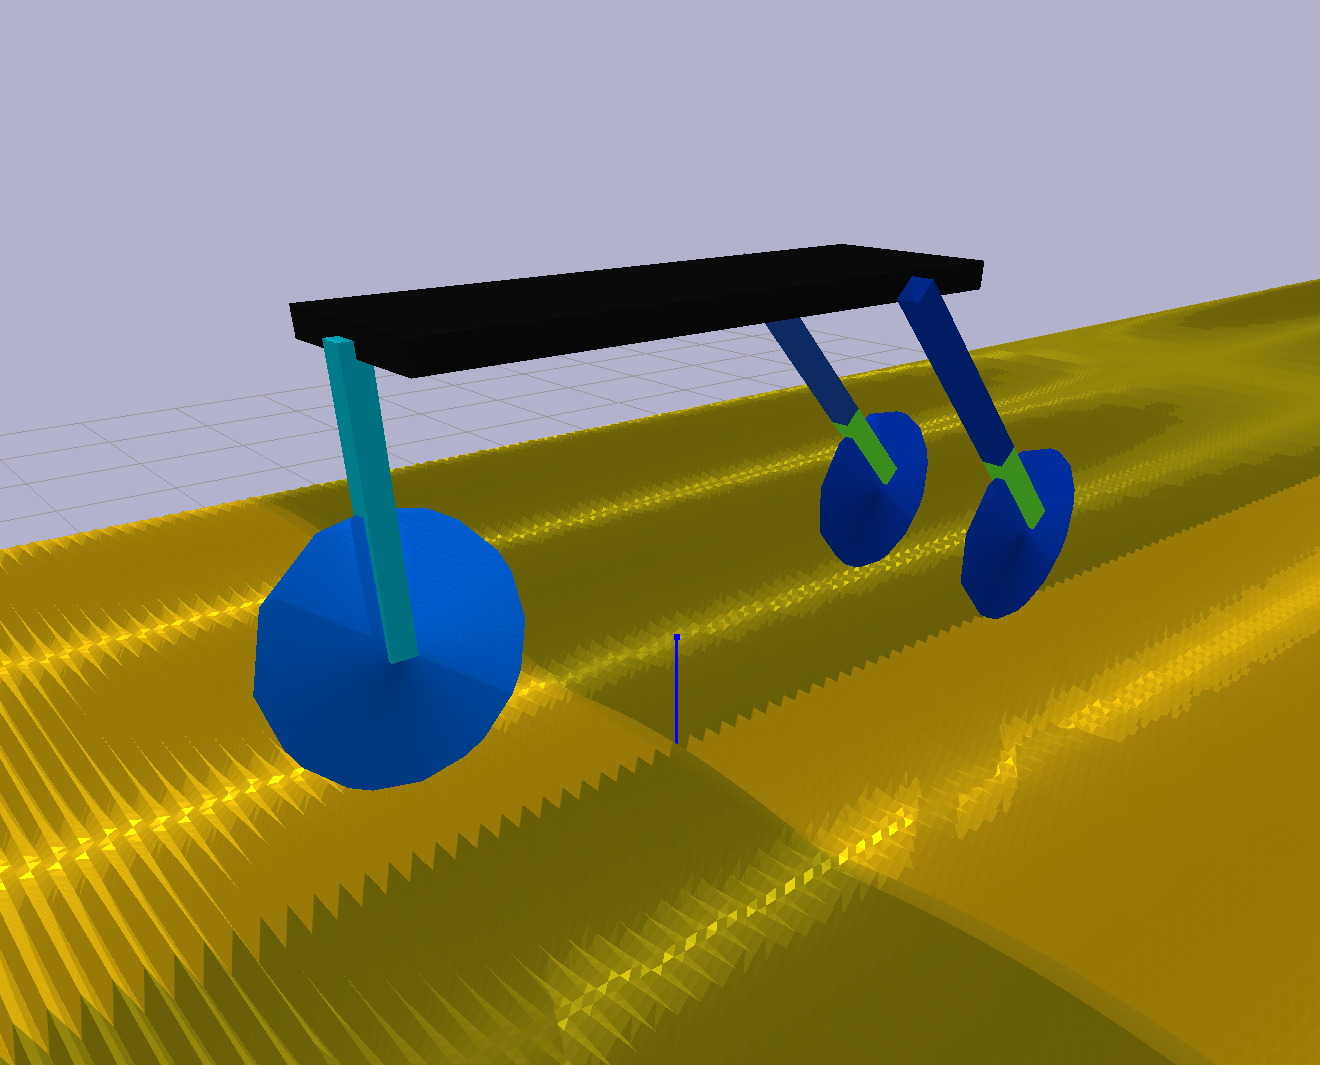
\includegraphics[width=\linewidth]{Figures/ch8_PivotThreeWheel.png}
        \caption{Three Wheeler With Pivot Actuator}
    \end{subfigure}
    \hfill
    \begin{subfigure}[b]{0.45\linewidth}
        \centering
        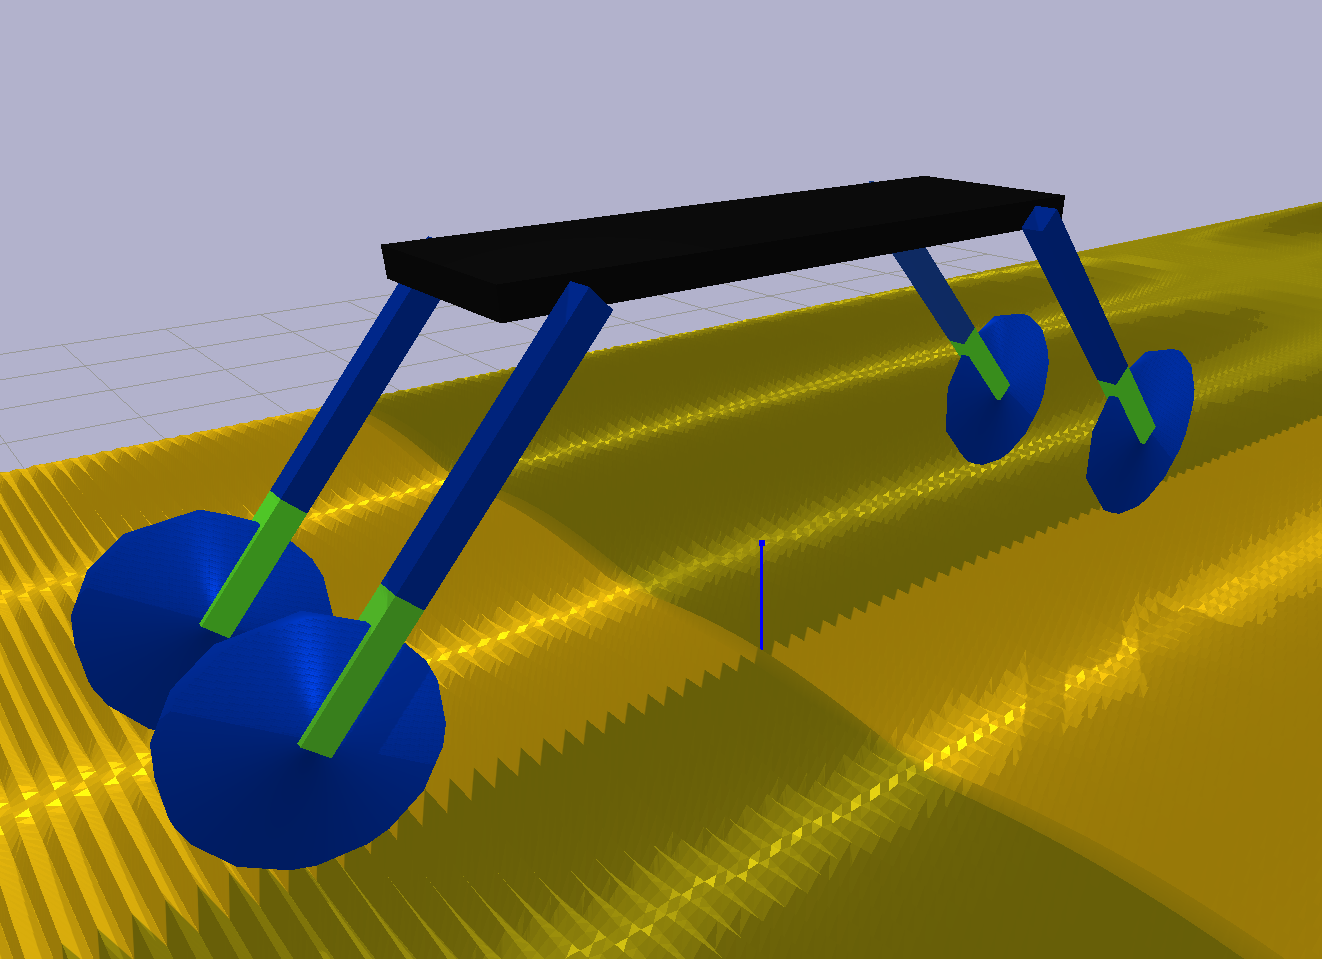
\includegraphics[width=\linewidth]{Figures/ch8_PivotFourWheel.png}
        \caption{Four Wheeler With Pivot Actuator}
    \end{subfigure}
    
    \caption{Comparison of Linear and Pivot Actuated Configurations for Three- and Four-Wheel Designs}
    \label{fig:actuator-configs}
\end{figure}

\subsection{Results}

To assess the dynamic behavior of each configuration, we evaluated their ability to maintain stability under straight-line and constant-radius turning using PID control. Below is a summary of the observed behavior for each of the four combinations of chassis layout (3-wheel vs. 4-wheel) and lean mechanism (pivot vs. linear actuator):

\begin{wrapfigure}{r}{0.45\linewidth}
    \centering
    \vspace{-1em}
    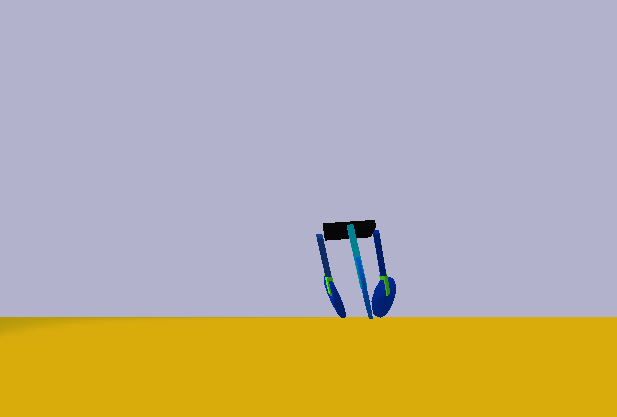
\includegraphics[width=\linewidth]{Figures/ch7_inwardWheel.png}
    \caption{Wheel inward locking behavior in pivot-based designs}
    \label{fig:wheel_instability}
    \vspace{-1em}
\end{wrapfigure}

In the pivot-based configurations, especially the 3-wheel version, we observed a strong tendency for wheels to lock inward or outward due to mass loading, as shown in Figure~\ref{fig:wheel_instability}. This arises from the geometry of the pivot as the mass of the cockpit press on the leg, which find a new minimum by having both wheel going inward or outward. If one try to mitigate the issue by increasing the spring constant of the wheel pivot, the vehicle is not able to turn smoothly and slip instead.

This behavior makes the pivot-based system unsuitable for high-speed or open-loop control. 

Furthermore, For both system, the \textit{mechanical trail} behind the pivot axis improves stability, which is consistent with known self-aligning behaviors in caster-like systems.

Both linear actuator variants (3- and 4-wheel) responded well to PID control in maintaining lean stability. Wheel wobble emerged at high speeds, particularly in the 3-wheel variant, but were manageable with increased damping and should likely be solved with a controller that will impact the wheel speed to create a cancelling moment. Both the three wheel and Four wheel linear actuator variant performed equally well. The four wheel variant as the advantage of allowing the loss of one of the actuator and thus offer some redunduncy. 

Figure~\ref{fig:linear_success_turn} and Figure~\ref{fig:fourwheel_success} show that it's possible to stabilize a steady state turn of the linear actuator based lean control during steady-state turning and straight line driving.

The plot showing the position, speed, acceleration of each element did not yield much result except to help tune the PID by looking at the response.
\begin{figure}[h!]
    \centering
    \begin{subfigure}[b]{0.48\linewidth}
        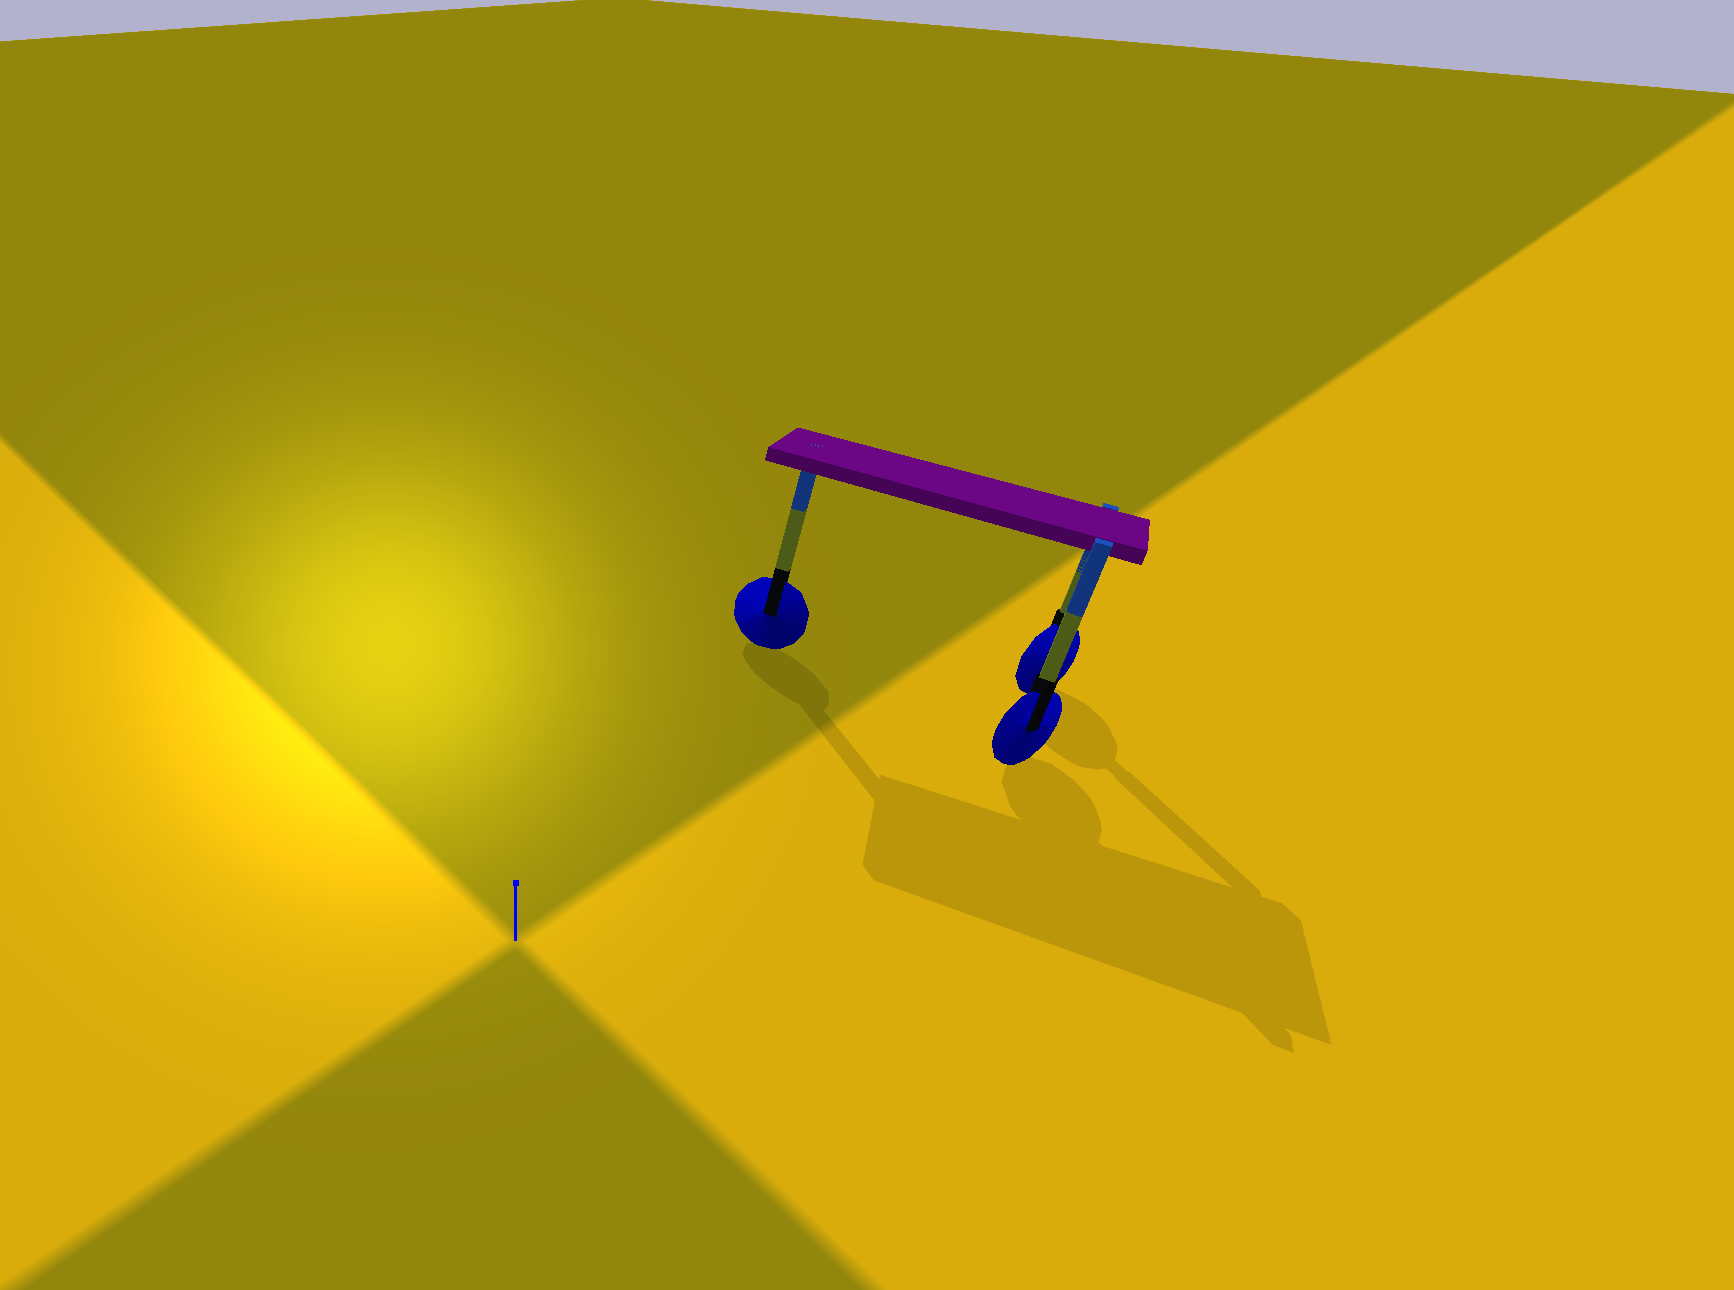
\includegraphics[width=\linewidth]{Figures/ch8_ThreeWheelLinearTurning.png}
        \caption{Three-wheel linear actuator turning}
        \label{fig:linear_success_turn}
    \end{subfigure}
    \hfill
    \begin{subfigure}[b]{0.48\linewidth}
        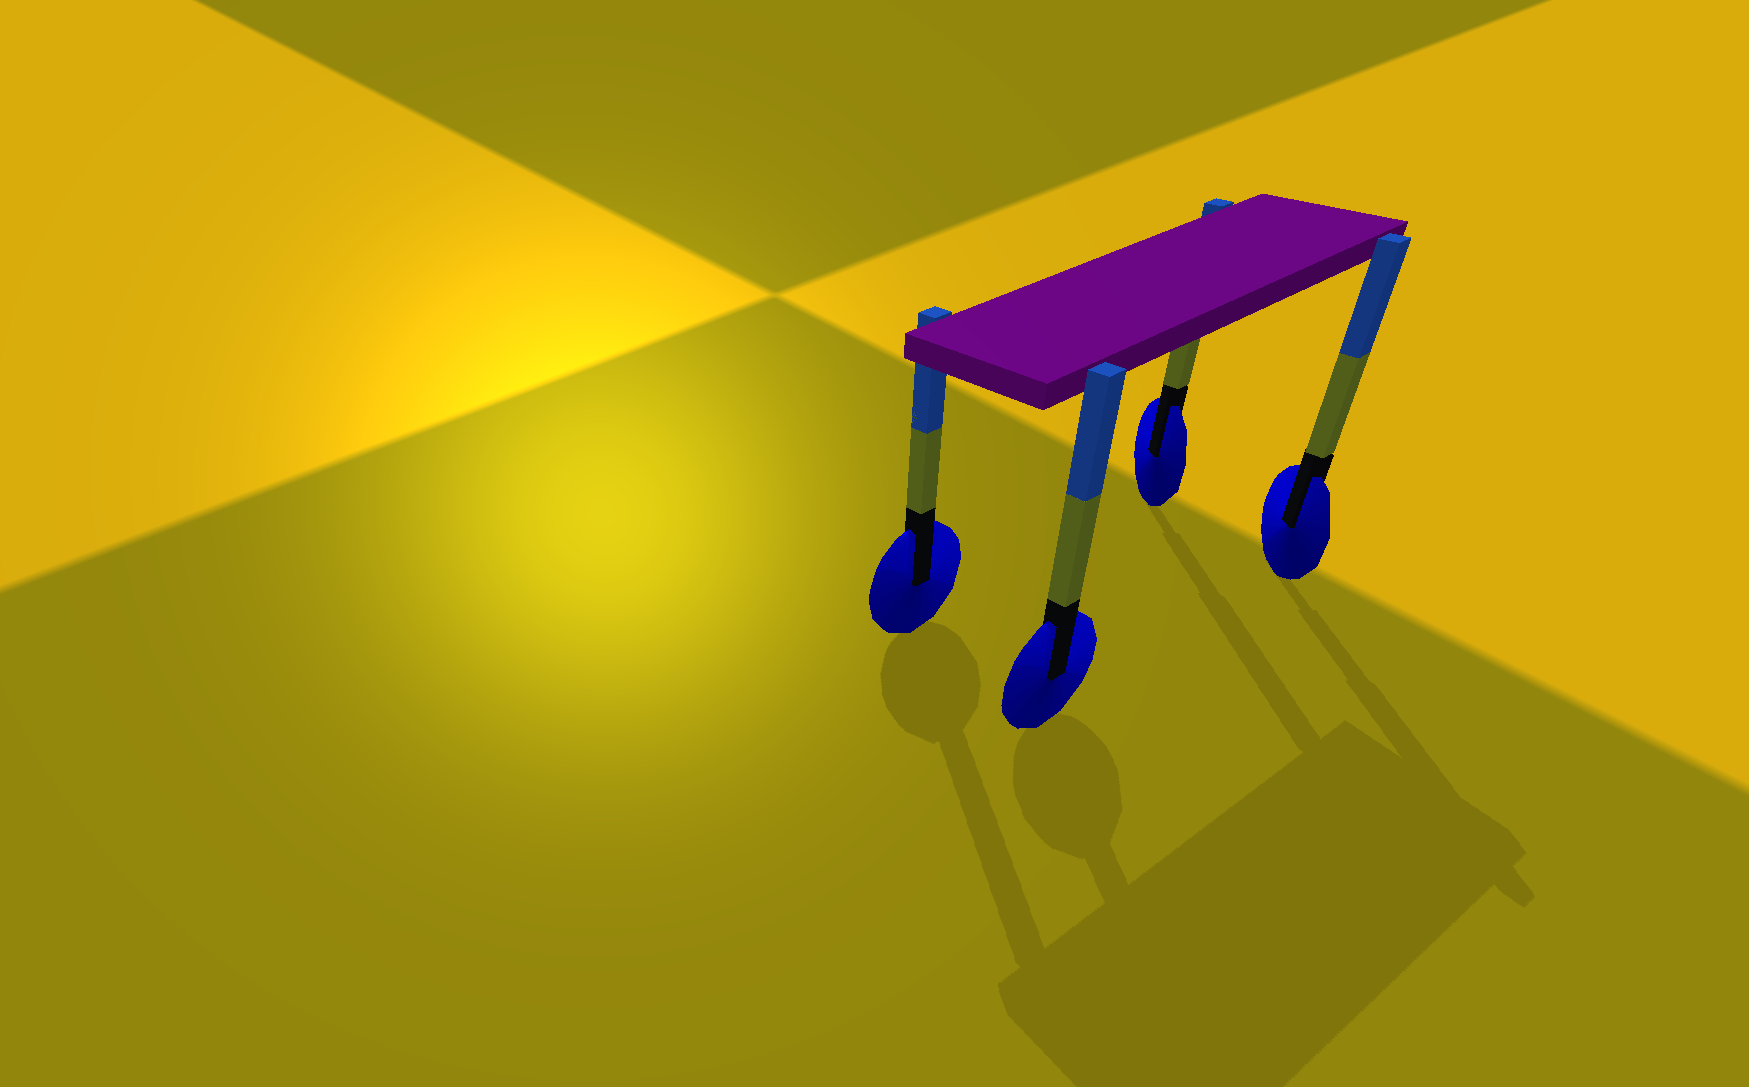
\includegraphics[width=\linewidth]{Figures/ch8_FourWheelSuccessfullTurn.png}
        \caption{Four-wheel linear actuator turning}
        \label{fig:fourwheel_success}
    \end{subfigure}
    \caption{Successful steady-state turning in linear actuator configurations}
\end{figure}

\begin{table}[h!]
\centering
\begin{tabular}{|c|c|c|}
\hline
\textbf{} & \textbf{Pivot Mechanism} & \textbf{Linear Actuator} \\
\hline
\textbf{3-Wheel} & 
\begin{tabular}[c]{@{}l@{}}
- Inherent instability in wheel alignment\\
- Wheels tend to lock inward/outward\\
- Trail effect offers some self-correction\\
- Poor turn stability without speed control
\end{tabular}
&
\begin{tabular}[c]{@{}l@{}}
- Stable under moderate speed\\
- Lean control effective with PID\\
- Wheel oscillation at high speed\\
- Responsive to speed vectoring
\end{tabular}
\\
\hline
\textbf{4-Wheel} & 
\begin{tabular}[c]{@{}l@{}}
- Only 2 passive pivoting wheels allowed\\
- Otherwise becomes uncontrollable\\
- Self-alignment is weak\\
- Strong inward force on wheels
\end{tabular}
& 
\begin{tabular}[c]{@{}l@{}}
- Most stable configuration\\
- Smooth turn response with PID\\
- Capable of steady-state turning\\
- Requires speed differential control
\end{tabular}
\\
\hline
\end{tabular}
\caption{Qualitative behavior observed in the four configurations}
\label{tab:design-summary}
\end{table}

These results suggest that a high-CoM tilting vehicle can be stabilized, provided the mechanical layout don't add too many non-linear coupling and independent wheel speed control is available.

\section{Conclusion and Future Work}

\subsection{Summary of Findings}

\subsection{Challenges and Limitations}

\subsection{Suggestions for Future Research}

compare the proposed geometry to the more "classic" one to see if it's more than good enough to work but at least as good or better than the classic design.

a prototype should be built to verify the theoretical model.

Safety in case of collisions should be integrated

if such vehicle was deployed, how would traffic look like inside the city ? would it help with congestion ? 
impact of trip time if we remonter la file au feux ? safety impact ?

Multi-Modal Transport Efficiency with Train Onboarding, what would happen if we took the train with our ”bike++” to coverage long distance ?
\section{Conclusion and Future Work}

\subsection{Summary of Findings}

\subsection{Challenges and Limitations}

\subsection{Suggestions for Future Research}
\section{Appendix}

% Add appendices here, if there are any

\newpage
\bibliographystyle{plain} 
\bibliography{References}

\end{document}
